%=======================================================================
\chapter[Multi-paradigm programming in Prolog and Java]{Multi-paradigm program-\\ming in Prolog and Java}
\label{ch:mpp-in-java}
%=======================================================================

\tuprolog{} supports multi-paradigm (and multi-language) programming between Prolog and Java in a complete, four-dimensional way:

\begin{itemize}
  \item using Java from Prolog: \textit{JavaLibrary}
  \item using Prolog from Java: \textit{the Java API}
  \item augmenting Prolog via Java: \textit{developing new libraries}
  \item augmenting Java via Prolog: \textit{the P@J framework}
\end{itemize}

%-----------------------------------------------------------------------
\section{Using Java from Prolog: \textit{JavaLibrary}}
\label{sec:java-library}
%-----------------------------------------------------------------------
The first MPP dimension offered by \tuprolog{} is the ability to fully access Java resources (objects, classes, methods, etc) in a full-fledged yet straightforward way, completely avoiding the intricacies (object and method pre-declarations in some awkward syntax, pre-compilations, etc) that are often found in other Prolog systems.
%
The unique \tuprolog{} approach keeps the two computational models clearly separate, so that neither the Prolog nor the Java semantics is affected by the coexistence of the logical and imperative/object-oriented paradigms in the same program.
%
In this way, any Java package, library, etc. is immediately available to the Prolog world with no effort, according to the motto {``one library for all libraries''}. So, for instance, Swing classes can be easily exploited to build the graphical support of a Prolog program, and the same holds for JDBC to access databases, for the socket package to provide network access, for RMI to access remote Java objects, and so on.

The two basic bricks of JavaLibrary are:
\begin{itemize}
  \item the mapping between Java types and suitable Prolog types;
  \item the set of predicates to perform operations on Java objects.
\end{itemize}

%-----------------------------------
\subsection{Type mapping}
%-----------------------------------

The general mapping between Prolog types and Java types is summarized in Table \ref{tab:prolog-java-type-mapping}.

\begin{table}[h]
  \centering
  \begin{tabular}{|p{1.8cm}|p{4.7cm}|p{4.7cm}|}
  \hline
  \textit{Categories} & \textit{From Prolog to Java} & \textit{From Java to Prolog}\\
  \hline
  integers   & Prolog integers are mapped onto Java \texttt{int} or \texttt{long} types, as appropriate & all Java integer types are mapped onto Prolog (integer) numbers\\
  \hline
  reals      & Prolog reals are mapped onto Java \texttt{double} & all Java floating-point types are mapped onto Prolog (real) numbers\\
  \hline
  booleans   & N/A & Boolean Java values are mapped onto ad-hoc constants (\texttt{true} and \texttt{false})\\
  \hline
  strings    & Prolog atoms are mapped onto Java \texttt{String}s & Java \texttt{char}s and \texttt{String}s are mapped onto Prolog atoms\\
  \hline
  wildcards  & Prolog indifference (the \textit{any} variable (\_)) is mapped onto the Java \texttt{null} costant & The Java \texttt{null} value is mapped onto the Prolog \textit{any} variable (\_)\\
  \hline
  \end{tabular}
  \caption{Prolog/Java type mapping.}\label{tab:prolog-java-type-mapping}
\end{table}

\noindent Two aspects are worth highlighting:
\begin{itemize}
  \item although the Prolog language considers a comprehensive \texttt{number} type for both integer and real values, the two kinds are considered separately in this table, both for the user's convenience and because \tuprolog{} internally does use different types for this purpose (indeed, the \tuprolog{} internal representation of numbers does distinguish \texttt{Number} into \texttt{Int}, \texttt{Long}, \texttt{Double} and \texttt{Float}, based on the value to be stored---details in Section \ref{ssec:java-api-types}).
      More precisely, in the Prolog-to-Java direction, only the Java \texttt{int}, \texttt{long} and \texttt{double} types are used as target types for the mapping, while in the opposite Java-to-Prolog direction any of the numeric Java types are accepted (including \texttt{short}, \texttt{byte} and \texttt{float}) for mapping onto Prolog numbers.
  \item since the Prolog language does not include a specific boolean type, the table reports N/A in the Prolog-to-Java direction; however, the \texttt{true} and \texttt{false} atoms can be provided to Java methods when appropriate, as Java boolean methods return/accept these atoms when boolean values are involved.
\end{itemize}

%---------------------------------------------------------------
\subsection{Creating and accessing objects: an overview}
\label{ssec:creating-and-accessing-objects}
%---------------------------------------------------------------

JavaLibrary provides many predicates to access, manipulate and interact with Java objects and classes in a complete way.
In this section, the fundamental predicates are presented that enable the Prolog user to create and access Java objects---that is, calling methods and getting return values.
A detailed description of all the available features is reported in Section \ref{ssec:all-javalibrary-predicates}.

For the sake of concreteness, Table \ref{tab:javalibrary-counter-example} reports a simple Java class (a counter) and the Prolog program that exploits it via JavaLibrary.

\begin{description}
  \item [Object creation]
        Java objects are created via the predicate

        \texttt{~~~~~java\_object(%
                 \textit{ClassName}, \textit{ArgList}, \textit{ObjRef} [,\textit{PathList}])}

        where \texttt{\textit{ClassName}} is a Prolog atom bound to the name of the
        Java class (e.g. \verb|'Counter'|, \verb|'java.io.FileInputStream'|, etc.), \texttt{\textit{ArgList}} is a Prolog list supplying the required arguments to the class constructor (the empty list matches the default constructor), and \texttt{\textit{ObjRef}} holds the reference to the newly-created object.
        In the case of arrays, \texttt{\textit{ClassName}} ends with \texttt{[]}.

        Optionally, a \texttt{\textit{PathList}} can be specified, enabling the dynamic class loading from virtually any path.
        Coherently with the lifetime of Prolog bindings, such paths only affect the specific \texttt{java\_object} call where
        they appear, being discarded immediately after. For the user convenience, the following syntactic conventions apply:
        \begin{itemize}
          \item any path entry ending with \texttt{'/'} or \texttt{$\backslash$} is supposed to be a \textit{prefix} of the class name;
          \item any path entry ending with \texttt{'.jar'} is supposed to be a JAR archive.
        \end{itemize}
        \noindent So, an entry like \texttt{'foo/bar/'} causes the \tuprolog{} class loader to look for \texttt{foo/bar/\textit{classname}.class}, while an entry like \texttt{'mylib.jar'} causes the
        \tuprolog{} class loader to look for \texttt{\textit{classname}.class} in the specified JAR.
        %
        In order to prevent a lot of boilerplate code to be unnecessarily repeated when the same paths are used often, the \texttt{set\_classpath/1} and \texttt{get\_classpath/1} predicates are also available (see below for details), which
        set the given path list into a \tuprolog{} engine permanently; so, if the required paths have been set via
        \texttt{set\_classpath/1}, the standard \texttt{java\_object/3} predicate can be used transparently, with no need
        of any further path specification---it will automatically look for classes in the specified paths.
        %
        Please note that such a permanent setting also affects the other JavaLibrary predicates, such as \texttt{as/2} (cast),
        array predicates, etc.

        The reference to the newly-created object is bound to \texttt{\textit{ObjRef}},
        which is typically a ground Prolog term; alternatively, an unbound term
        may be used, in which case the term is bound to an automatically-generated
        Prolog atom of the form \verb|'$obj_N'|, where \texttt{N} is an integer.

        In both cases, these atoms are interpreted as object references --
        and therefore used to operate on the Java object from Prolog -- \textit{only} in the context of \texttt{JavaLibrary}'s predicates: this is how \tuprolog{} guarantees that the two computational models are never mixed, and therefore that each semantics is preserved.

        The predicate fails if \texttt{\textit{ClassName}} does not identify a valid Java class, or the constructor does not exists, or arguments in
        \texttt{\textit{ArgList}} are not ground, or \textit{ObjRef}
        already identifies another object in the system.

        The lifetime of the binding between the Java object and the Prolog term
        is the duration of the demonstration: by default, the binding is maintained in case of backtracking, but this behavior can be changed by setting the flag \texttt{java\_object\_backtrackable} flag to \texttt{true}.

        To make such a binding permanent, that is, to ``keep alive'' the binding between a Java object and a Prolog term beyond the current query, so as to exploit it in another, subsequent demonstration, the \texttt{register/1} predicate is provided (new in \tuprolog{} 2.6), along with its \texttt{unregister/1} counterpart;
        this can also be done on the Java side, via the \tuprolog{} Java API.
        However, this feature should not be abused: generally speaking, when operating from the Prolog side, objects needed by other predicates (within the same demonstration) should be passed over as arguments, coherently with the Prolog philosophy of avoiding any global side effect (except for \texttt{assert} predicates).

  \item [method calling]
        methods can be invoked on Java objects via the \texttt{<-/2} predicate,
        according to a send-message pattern. The predicate comes in two flavors, with/without return argument:

        \texttt{~~~~~\textit{ObjectRef} <- \textit{MethodName}(\textit{Arguments})}

        \texttt{~~~~~\textit{ObjectRef} <- \textit{MethodName}(\textit{Arguments})
                returns \textit{Term}}

        where \texttt{\textit{ObjectRef}} is an atom interpreted as a Java object
        reference as above, and \texttt{\textit{MethodName}} is the Java name of the method to be invoked, along with its \texttt{\textit{Arguments}}.

        The \texttt{returns} keyword is used to retrieve the value returned from non-void Java methods and bind it to a Prolog term: if the type of the returned value can be mapped onto a primitive Prolog data type (a number or a string), \texttt{\textit{Term}} is unified with the corresponding Prolog value; otherwise, \texttt{\textit{Term}} is handled as an object reference, that is, as a Prolog ground term\footnote{If it is not ground, it is automatically bound to a term like \texttt{\$obj\_N}.} bound to the Java object returned by the method.

        Static methods can also be invoked, specifying one of the special terms \texttt{class(\textit{ClassName})} or \texttt{class(\textit{ClassName},\textit{PathList})} as the target \texttt{\textit{ObjRef}}.
        As above, the optional \texttt{\textit{PathList}} argument specifies the paths where to search the classes to be loaded.

        The call fails if \texttt{\textit{MethodName}} does not identify a valid method for the object (for the class, in the case of static methods), or arguments in \texttt{\textit{ArgList}} are invalid because of a wrong signature or because they are not ground.

  \item [property selection]
        public object properties can be accessed via the \texttt{.} infix operator, in conjunction with the \texttt{set} / \texttt{get} pseudo-method pair:

        \texttt{~~~~~\textit{ObjectRef}.\textit{Field} <- set(\textit{GroundTerm})}

        \texttt{~~~~~\textit{ObjectRef}.\textit{Field} <- get(\textit{Term})}

        The first construct sets the public field \texttt{\textit{Field}} to the specified \texttt{\textit{GroundTerm}}, which may be either a value of a primitive data type, or a reference to an existing object: if it is not ground, the infix predicate fails.

        Analogously, the second construct retrieves the value of the public field
        \texttt{\textit{Field}}, handling the returned \texttt{\textit{Term}} as above.

        Again, class properties can be accessed using the  \texttt{class(\textit{ClassName})} form for  \texttt{\textit{ObjectRef}}.

        It is worth to point out that such \texttt{set} / \texttt{get}
        pseudo-methods are \textit{not} methods of some class, but just
        part of of the property selection operator.

  \item [array access]
        Due to the special Java syntax for arrays, ad hoc helper predicates are required to access Java array elements:

        \texttt{~~~~~java\_array\_set(\textit{ArrayRef}, \textit{Index}, \textit{Object})}

        \texttt{~~~~~java\_array\_get(\textit{ArrayRef}, \textit{Index}, \textit{Object})}

        \texttt{~~~~~java\_array\_set\_\textit{\emph{Basic Type}}(\textit{ArrayRef}, \textit{Index}, \textit{Value})}

        \texttt{~~~~~java\_array\_get\_\textit{\emph{Basic Type}}(\textit{ArrayRef}, \textit{Index}, \textit{Value})}

        \texttt{~~~~~java\_array\_length(\textit{ArrayObject}, \textit{Size})}

  \item [type cast]
        the \texttt{as} infix operator is used to explicitly cast method arguments to a given type, typically for exploiting overloading resolution:

        \texttt{~~~~~\textit{ObjectRef} as \textit{Type}}

        By writing so, the object represented by \texttt{\textit{ObjectRef}} is considered to belong to type \texttt{\textit{Type}}: the latter can be either a class name, as above, or a primitive Java type such as \texttt{int}.

  \item [classpath specification, class loading and dynamic compilation]

        The \texttt{set\_classpath/1} and \texttt{get\_classpath/1} respectively sets/gets the given path list into a \tuprolog{} engine permanently; accordingly, after a path has been set via \texttt{set\_classpath/1}, all the JavaLibrary predicates (object creation, method calling, etc) can be used transparently, with no need of any further path specification.

        The \texttt{java\_class/4} creates, compiles and loads a new Java class from a source text:

        \texttt{~~~~~java\_class(\textit{SourceText}, \textit{FullClassName},}\\
        \texttt{\mbox{~~~~~~~~~~~~~~~~}\textit{PathList}, \textit{ObjectRef})}

        where \texttt{\textit{SourceText}} is a string representing the text source of the new Java class, \texttt{\textit{FullClassName}} is the full class name, and \texttt{\textit{PathList}} is a (possibly empty) Prolog list of class paths that may be required for a successful dynamic compilation of this class.
        %
        In this case, \texttt{\textit{ObjectRef}} is a reference to an instance of the meta-class \texttt{java.lang.Class} representing the newly-created class.

        The predicate fails if \texttt{\textit{SourceText}} leads to compilation errors, or the class cannot be located in the package hierarchy, or \texttt{\textit{ObjectRef}} already identifies another object in the system.
\end{description}

\noindent Exceptions thrown by Java methods or constructors can be managed by means of \tuprolog{}'s special \texttt{java\_catch} %and \texttt{java\_throw} predicates,
predicate, discussed in Section \ref{ssec:java-exceptions-in-tuprolog}.

%------------------------
\subsubsection{Examples}
%------------------------

\begin{table}
\textit{Java class:}
\begin{verbatim}
public class Counter {
    public String name;
    private long value = 0;

    public Counter() {}
    public Counter(String aName) { name = aName; }

    public void setValue(long val) { value=val; }
    public long getValue() { return value; }
    public void inc() { value++; }

    static public String getVersion() { return "1.0"; }
}
\end{verbatim}

\textit{Prolog program:}
\begin{verbatim}
    ?-  java_object('Counter', ['MyCounter'], myCounter),

        myCounter <- setValue(5),
        myCounter <- inc,
        myCounter <- getValue returns Value,
        write(Value), nl,

        class('Counter') <- getVersion return Version,
        write(Version), nl,

        myCounter.name <- get(Name),
        class('java.lang.System') . out <- get(Out),
        Out <- println(Name),

        myCounter.name <- set('MyCounter2'),

        java_object('Counter[]', [10], ArrayCounters),
        java_array_set(ArrayCounters, 0, myCounter).
\end{verbatim}
\caption{The Java \texttt{Counter} class and the Prolog program that exploits it via JavaLibrary.}
\label{tab:javalibrary-counter-example}
\end{table}

To taste the flavor of \texttt{JavaLibrary}, let us consider the example shown in Table \ref{tab:javalibrary-counter-example}, which reports both a simple Java class (a counter) and the Prolog program that exploits it via JavaLibrary.

First, a \texttt{Counter} instance is created (line 1) providing the \texttt{MyCounter} name as the constructor argument: the reference to the new object is bound to the Prolog atom \texttt{myCounter}.

Then, this reference is used to invoke several methods (lines 2--4) via the \verb|<-/2| and the (\verb|<-|,\texttt{returns})\texttt{/3} operators---namely, \texttt{setValue(5)} (which is void and therefore returns nothing), \texttt{inc} (which takes no arguments and is void, too) and \texttt{getValue} (which takes no argument but returns an int value);
the returned value (hopefully, 5) is bound to the \texttt{X} Prolog variable, which is finally printed via the Prolog \texttt{write/1} predicate (line 5).
%
Of course, the predicate succeeds also if \texttt{X} is already bound to 5, while fails if it is already bound to anything else.

Then, the class (static) method \texttt{getVersion} is called (line 6) and the retrieved version number is printed (line 7).

Now the (public) instance \textit{\texttt{Name}} property is read, and its value printed via the Java \texttt{System.out.println} method: to this end, a reference to the \texttt{java.lang.System} class is first obtained (line 8), then its \texttt{out} (static) field is accessed and its value retrieved and bound to the \texttt{Out} Prolog variable (line 9), which is used as the target for the invocation of the \texttt{println} method (line 10).

Finally, the \texttt{name} property of the \texttt{myCounter} object is changed to the new \texttt{'MyCounter2'} value (line 11).

The last part of the example deals with an array of 10 \texttt{Counter}s: the array is first created (line 12), and the \texttt{myCounter} object is assigned to its first (0th) element (line 13).

The key point is that the only requirement here is the presence of the \texttt{Counter.class} file in the proper location in the file system, according to Java naming conventions: no other auxiliary information is needed---no headers, no pre-declarations, pre-compilations, etc.

%------------------

Table \ref{tab:jexamples-swing} shows one further example, where the Java Swing API is
exploited to graphically choose a file from Prolog: a Swing \texttt{JFileChooser} dialog is instantiated and bound to the Prolog variable \texttt{Dialog} (a univocal Prolog atom of the form \verb|'$obj_N'|, to be used as the object reference, is automatically generated and bound to that variable) and is then used to invoke the \texttt{showOpenDialog} and
\texttt{getSelectedFile} methods: the Prolog anonymous variable \texttt{\_} is used to represent the Java \texttt{null} value in \texttt{showOpenDialog}.
%
The \texttt{File} object returned by the file chooser is finally queries for the corresponding \texttt{FileName}, which is returned to the outer predicate caller.

%Further examples about exploiting standard Java libraries from \tuprolog{} can be found in \cite{tuprolog-padl2001} and \cite{tuprolog-scico2005}.

\begin{table}
\begin{verbatim}
test_open_file_dialog(FileName) :-
    java_object('javax.swing.JFileChooser', [], Dialog),
    Dialog <- showOpenDialog(_),
    Dialog <- getSelectedFile returns File,
    File <- getName returns FileName.
\end{verbatim}
\caption{Creating and using a Swing component from a \tuprolog{} program.}
\label{tab:jexamples-swing}
\end{table}

%-----------------------------------------------------------------------
\subsubsection{Registering object bindings}
\label{sssec:register(prolog)}
%-----------------------------------------------------------------------

As explained above, the standard lifetime of the binding between Java objects and Prolog atoms is that of the current demonstration, in coherence with the lifetime of Prolog variable bindings.
However, some multi-paradigm applications may require that a Java object is maintained alive and retrieved later without passing it along as an argument throughout the program: this is what the \texttt{register} predicate is for.
Its syntax is as follows:\\

\texttt{~~~~~register(\textit{ObjectRef})}\\

\noindent where \texttt{\textit{ObjectRef}} is already bound to some Java object. The effect is to make such binding survive the current demonstration, until the dual \texttt{unregister} predicate is possibly called:\\

\texttt{~~~~~unregister(\textit{ObjectRef})}\\

\noindent The requirement that \texttt{\textit{ObjectRef}} is already bound to some Java object inherently excludes pre-existing, non-public Java objects from being registered, since the only ways to establish a binding between a Prolog atom and a Java object from the Prolog side are the \texttt{java\_object} predicate, which creates a new instance, and the property selection operator (\texttt{.},\texttt{<-get(\textit{Name})}), which accesses public properties.
%
Public Java objects, including the static ones like \texttt{System.out}, can instead be registered by retrieving a reference to their binding first---as in the example shown in Table \ref{tab:javalibrary-counter-example} above, where a reference to \texttt{System.out} is retrieved to call the \texttt{println} method.

Binding registration can be performed also on the Java side, as detailed in Section \ref{ssec:register(Java)}.

%---------------------------------------------------------------------
\subsection{Predicates}
\label{ssec:all-javalibrary-predicates}
%---------------------------------------------------------------------

The following predicate description details all the JavaLibrary predicates: a summary overview is also reported in Table \ref{tab:summary-of-javalibrary-predicates}.
%
Throughout this Section, only the exceptions specifically related to the JavaLibrary predicates' behaviors are listed: other exceptions might obviously occur, based on the exceptions possibly raised by the invoked method, which can not be foreseen in any way.

\begin{table}
    \begin{center}{\scriptsize
    \begin{tabular}{p{2.3cm}p{6.6cm}p{4.6cm}}\hline\hline
    \\
    %--------------------------------------------------------------------------
    {\small \textbf{Functionality}} &
    {\small \textbf{Predicate(s)}} &
    {\small \textbf{Description}}
    \\\\\hline\\
    %--------------------------------------------------------------------------
    Object creation
    &
    \texttt{java\_object(+\textit{ClassName}, +\textit{ArgList}, ?\textit{ObjRef})}\newline
    \texttt{java\_object(+\textit{ClassName}, +\textit{ArgList}, ?\textit{ObjRef},
    \mbox{~~~~~~~~~~~~~~~~~~~~~~~~~~~~~~~~}+\textit{PathList})}\newline
    \texttt{java\_object(+\textit{ClassName}[], [+\textit{Len}], ?\textit{ObjRef})}
    \newline
    \newline
    Examples:\newline
    \texttt{java\_object(`java.awt.Point', [2,3], P)}\newline
    \texttt{java\_object(`java.lang.Integer', [303], n)}\newline
    \texttt{java\_object(`java.awt.Point'[], [100], V)}
    &
    Creates a Java object of class \textit{\texttt{ClassName}} calling the
    constructor matching the arguments in \textit{\texttt{ArgList}}; if
    \textit{\texttt{ClassName}} is followed by \texttt{[]}, an array is created.
    The class \textit{\texttt{ClassName}} must be either in the current class path or
    in the paths specified in \texttt{\textit{PathList}}.
    On success, \textit{\texttt{ObjRef}} is bound to a term representing the
    object: if it was a variable, it is bound to a system-generated atom
    of the form \texttt{\$obj\_\textit{N}}.
    \\\\\hline\\
    %--------------------------------------------------------------------------
    Method\newline invocation
    &
    \textit{\texttt{TargetRef}} \verb <- ~\texttt{\textit{MethodName}}\newline
    \textit{\texttt{TargetRef}} \verb <- ~\texttt{\textit{MethodName}(+\textit{Arg0},+\textit{Arg1},\ldots)}\newline
    \textit{\texttt{TargetRef}} \verb <- ~\texttt{\textit{MethodName} returns \textit{Res}}\newline
    \textit{\texttt{TargetRef}} \verb <- ~\texttt{\textit{MethodName}(+\textit{Arg0},+\textit{Arg1},\ldots)\newline
    \mbox{~~~~~~~~~~~~~~~~~~~~~~~~}returns \textit{Res}}
    \newline
    Example 1:\newline
    \texttt{java\_object(`java.awt.Point', [2,3], P),}\newline
    \texttt{P} \verb <- ~\texttt{getX returns X}\newline
    Example 2:\newline
    \texttt{Intclass = class(`java.lang.Integer')}\newline
    \texttt{Intclass} \verb <- ~\texttt{parseInt(`200') returns N}
    &
    Invokes the method \textit{\texttt{MethodName}} on the object associated
    to the \textit{\texttt{TargetRef}} term, possibly passing arguments
    \textit{\texttt{Arg0}}, \textit{\texttt{Arg1}}, etc., and possibly binding
    the return argument to the \texttt{\textit{Res}} term.
    \newline
    Static methods are invoked using \texttt{class(\textit{ClassName})}
    or \texttt{class(\textit{ClassName}, \textit{PathList})}
    as \texttt{\textit{TargetRef}}.
    \\\\\hline\\
    %--------------------------------------------------------------------------
    Field (property) access
    &
    \texttt{\textit{TargetRef} . \textit{FieldName}} \verb <- ~\texttt{set(+\textit{Arg})}\newline
    \texttt{\textit{TargetRef} . \textit{FieldName}} \verb <- ~\texttt{get(+\textit{Arg})}\newline
    \newline
    &
    Accesses the public field (property) \texttt{\textit{FieldName}} of object
    \texttt{\textit{TargetRef}} to set/get its value to the
    value (or object reference) denoted by \texttt{\textit{Arg}}.
    %
    For static fields, the compound term \texttt{class(\textit{ClassName})}
    shall be used as \texttt{\textit{TargetRef}}.
    \\\\\hline\\
    %--------------------------------------------------------------------------
    Array access\newline and management
    &
    \texttt{java\_array\_set(+\textit{ArrayRef}, +\textit{Pos}, +\textit{Content})}\newline
    \texttt{java\_array\_get(+\textit{ArrayRef}, +\textit{Pos}, ?\textit{Content})}\newline
    \texttt{java\_array\_length(+\textit{ArrayRef}, ?\textit{Length})}\newline
    \newline
    Example:\newline
    \texttt{java\_object(`java.awt.Point'[], [100], V),}\newline
    \texttt{java\_object(`java.awt.Point', [1,2], Point),}\newline
    \texttt{java\_array\_set(A, 0, Point)}
    &
    Accesses position \texttt{\textit{Pos}} of the array bound to the
    \texttt{\textit{ArrayRef}} term to set/get the content of that position
    to the value (or object reference) associated to the \texttt{\textit{Content}} term.
    \newline
    The third predicate retrieves the array length and binds it to the
    \textit{\texttt{Length}} term.
    \\\\\hline\\
    %--------------------------------------------------------------------------
    Cast
    &
    \texttt{\textit{Arg} as \textit{TypeName}}\newline
    &
    Forces argument \texttt{\textit{Arg}} to be considered of type
    \texttt{\textit{TypeName}}.
    \\\\\hline\\
    %--------------------------------------------------------------------------
    Dynamic class \newline compilation
    &
    \texttt{java\_class(+\textit{Source}, +\textit{ClassName},}\newline
    \mbox{~~~~~~~~~~~~~~~~}\texttt{+\textit{PathList}, ?\textit{ClassRef})}\newline
    &
    Dynamically compiles the source text \texttt{\textit{Source}}
    to define the new class named \texttt{\textit{ClassName}}.
    \texttt{\textit{PathList}} denotes the class path to be used
    for compilation.
    The compiled class, available as a \texttt{Class} instance,
    is associated to the \texttt{\textit{ClassRef}} term.
    \\
    %--------------------------------------------------------------------------
    \\
    \hline\hline
    \end{tabular}
    }\end{center}
    \caption{Summary of \texttt{JavaLibrary} predicates.}
    \label{tab:summary-of-javalibrary-predicates}
\end{table}

%---------------------------------------------------------------------
\subsubsection{Object creation, class compilation and method invocation}
%---------------------------------------------------------------------

\begin{itemize}

\item \bti{java\_object/3} and \bti{java\_object/4}\\
    \noindent \bt{java\_object(\textit{ClassName}, \textit{ArgList}, \textit{ObjectRef})} instantiates a new instance of class \bt{\textit{ClassName}} (full class name on the current class path) and initializes it via the Java constructor matching the arguments in \bt{\textit{ArgList}}; the newly created Java object is bound to the Prolog term \bt{\textit{ObjectRef}}, which can be any ground term (except for numbers) or a Prolog variable (in which case it is bound to an  automatically-generated ground term).
    By default, such a binding is \textit{not} undone on backtracking, unless the \texttt{java\_object\_backtrackable} flag is set to \texttt{true} (see Section \ref{ssec:creating-and-accessing-objects}).
    The \bti{java\_object/4} version takes a path list as an extra argument: such paths are also looked for the class file, in addition to the standard class path.

    \template{java\_object(+class\_name, +arg\_list, ?object\_ref)}

    \template{java\_object(+class\_name, +arg\_list, ?object\_ref, \\
    \mbox{~~~~~~~~~~~~~~~~~~~~~~~~~~~~~~~~~~~~~~~~~~~~~~~}+path\_list)}

    \exception{java.lang.ClassNotFoundException(Cause, Message, StackTrace)} if \bt{ClassName} does not identify a valid class name on the local file system.

    \exception{java.lang.NoSuchMethodException(Cause, Message, \\StackTrace)} if the specified constructor could not be found.

    \exception{java.lang.reflect.InvocationTargetException(Cause, Message, StackTrace)} if the constructor arguments are invalid---for instance, because they are not ground.

    \exception{java.lang.Exception(Cause, Message, StackTrace)} if \texttt{ObjectRef} is already bound to another Java object.


\item \bti{java\_object\_bt/3} and \bti{java\_object\_bt/4}\\
    everything as above, but the binding \textit{is} undone on backtracking.

\item \bti{destroy\_object/1}\\
    \noindent\bt{destroy\_object(ObjectRef)} removes the binding possibly established between \bt{ObjectRef} and an underlying Java object.

    \template{destroy\_object(@object\_ref)}

\item \bti{java\_class/4}\\
    \noindent\bt{java\_class(SourceText, ClassName, PathList, ObjectRef)}
    creates the new Java class \texttt{ClassName} from the provided \texttt{\textit{SourceText}}, compiles it dynamically using to the classes in the provided \bt{PathList}, and binds the result -- a suitable instance of the meta-class \texttt{Class} -- with the Prolog term \bt{ObjectRef}.

    \template{java\_class(@source, @classname, @path, ?obj\_ref)}

    \exception{java.lang.ClassNotFoundException(Cause, Message, StackTrace)} if \bt{ClassName} does not identify a valid class name in the package hierarchy on the local file system.

    \exception{java.lang.IOException(Cause, Message, StackTrace)} if \texttt{\textit{SourceText}} contains errors that prevent the class from being compiled.

    \exception{java.lang.Exception(Cause, Message, StackTrace)} if \texttt{ObjectRef} is already bound to another Java object.


\item \bti{java\_call/3}\\
    \noindent\bt{java\_call(ObjectRef, Method, ResultRef)} is the basic method implementing the infix \verb|<-/2| and (\verb|<-|,\texttt{returns})\texttt{/3} operators below. It is true iff \bt{ObjectRef} is a ground term bound to a Java object, and this provides a method \bt{Method} (that is, whose name is the functor name and whose arguments are the arguments of the compound term \bt{Method}); \bt{ResultRef} is a Prolog term bound to the returned value.
    \texttt{\textit{ObjectRef}} takes the form \texttt{class(\textit{ClassName})} or \texttt{class(\textit{ClassName}, \textit{PathList})} for static methods.

    If needed, the Prolog anonymous variable \texttt{\_} can be used as an argument for the Java \texttt{null} value.

    \template{java\_call(@obj\_id, @method\_signature, ?ResultRef)}

    \exception{java.lang.NoSuchMethodException(Cause, Message,\\
    StackTrace)} if the specified method could not be found in the target object/class, or the method arguments are invalid.

\item \verb|<-/2|\\
    \noindent\verb|ObjectRef <- Method| calls the Java method represented by the \texttt{Method} compound term on the target Java object \bt{ObjectRef}. The same argument specifications of \texttt{java\_call} above apply.

    \template{'<-'(@obj\_id, @method\_signature)}

    \exception{} as above

\item (\verb|<-|,\bti{returns})\texttt{/3}\\
    \noindent\verb|ObjectRef <- Method returns ResultRef| calls the Java method represented by the \texttt{Method} compound term on the target Java object \bt{ObjectRef}, retrieving the method result into \texttt{ResultRef}. The same argument specifications of \texttt{java\_call} above apply.

    Formally, this operator is defined as the binary \texttt{returns/2} predicate, whose first argument has the form of the above \verb|<-/2| predicate (see Table \ref{tab:javalibrary-operators} below for these operators' priorities).

    \template{returns('<-'(@obj\_id, @method\_signature), ?@obj\_id)}

    \exception{} as above
\end{itemize}

%---------------------------------------------------------------------
\subsubsection{Array management}
%---------------------------------------------------------------------
\begin{itemize}

\item the \bti{java\_array\_set\_*/3} family\\
    This family of predicates is composed of one main predicate handling arrays of objects, and a set of helper predicates handling arrays of primitive Java types.

    \bt{java\_array\_set(ArrayRef, Index, ObjectRef)} is the main predicate, setting the \texttt{Index}th cell of the array \texttt{ArrayRef} to \bt{ObjectRef} (i.e., \texttt{ArrayRef[Index]=ObjectRef}).
    So, \bt{ArrayRef} is a ground term referencing a Java array object, \bt{Index} is a valid 0-based index for that array, and \bt{ObjectRef} is a ground term bound to a Java object (of an assignment-compatible type according to the Java type rules) to be inserted into the array at the given position.
    As above, the Prolog anonymous variable can be used as \bt{ObjectRef} to denote the Java \texttt{null} value.

    Arrays of primitive Java types are handled analogously by the following set of helper predicates:

    \mbox{~~~~}\bt{java\_array\_set\_int(ArrayRef, Index, Integer)}\\
    \mbox{~~~~}\bt{java\_array\_set\_short(ArrayRef, Index, ShortInteger)}\\
    \mbox{~~~~}\bt{java\_array\_set\_long(ArrayRef, Index, LongInteger)}\\
    \mbox{~~~~}\bt{java\_array\_set\_float(ArrayRef, Index, Float)}\\
    \mbox{~~~~}\bt{java\_array\_set\_double(ArrayRef, Index, Double)}\\
    \mbox{~~~~}\bt{java\_array\_set\_char(ArrayRef, Index, Char)}\\
    \mbox{~~~~}\bt{java\_array\_set\_byte(ArrayRef, Index, Byte)}\\
    \mbox{~~~~}\bt{java\_array\_set\_boolean(ArrayRef, Index, Boolean)}

    \template{java\_array\_set(@obj\_id, @nonneg\_integer, +obj\_id)}

    \exception{java.lang.IllegalArgumentException(Cause, Message, StackTrace)} if the \texttt{ArrayRef} does not refer to a valid array object, or \texttt{Index} is incorrect, or \texttt{ObjectRef} is not type-assignable to the array.

\item the \bti{java\_array\_get\_*/3} family\\
    This family of predicates is composed of one main predicate handling arrays of objects, and a set of helper predicates handling arrays of primitive Java types.

    \bt{java\_array\_get(ArrayRef, Index, ObjectRef)} is the main predicate, getting the \texttt{Index}th cell of the array \texttt{ArrayRef} into \bt{ObjectRef} (i.e., \texttt{ObjectRef=ArrayRef[Index]}).
    So, \bt{ArrayRef} is a ground term referencing a Java array object, \bt{Index} is a valid 0-based index for that array, and \bt{ObjectRef} is a ground term unified with the reference to the Java object (of an assignment-compatible type according to the Java type rules) at the given array position.
    Again, the Prolog anonymous variable can be used as \bt{ObjectRef} to denote the Java \texttt{null} value.

    Arrays of primitive Java types are handled analogously by the following set of helper predicates:

    \mbox{~~~~}\bt{java\_array\_get\_int(ArrayRef, Index, Integer)}\\
    \mbox{~~~~}\bt{java\_array\_get\_short(ArrayRef, Index, ShortInteger)}\\
    \mbox{~~~~}\bt{java\_array\_get\_long(ArrayRef, Index, LongInteger)}\\
    \mbox{~~~~}\bt{java\_array\_get\_float(ArrayRef, Index, Float)}\\
    \mbox{~~~~}\bt{java\_array\_get\_double(ArrayRef, Index, Double)}\\
    \mbox{~~~~}\bt{java\_array\_get\_char(ArrayRef, Index, Char)}\\
    \mbox{~~~~}\bt{java\_array\_get\_byte(ArrayRef, Index, Byte)}\\
    \mbox{~~~~}\bt{java\_array\_get\_boolean(ArrayRef, Index, Boolean)}

    \template{java\_array\_get(@obj\_id, @nonneg\_integer, ?obj\_id)}

    \exception{java.lang.IllegalArgumentException(Cause, Message, StackTrace)} if the \texttt{ArrayRef} does not refer to a valid array object, or \texttt{Index} is incorrect.

\item \bti{java\_array\_length/2}\\
    \noindent\bt{java\_array\_length(ArrayRef, ArrayLength)} is true iff \bt{ArrayLength} is the length of the Java array referenced by
    the term \bt{ArrayRef}.

    \template{java\_array\_length(@term, ?integer)}
\end{itemize}

%---------------------------------------------------------------------
\subsubsection{Helper predicates}
%---------------------------------------------------------------------

\begin{itemize}
\item \bti{set\_classpath/1}\\
    \noindent\bt{set\_classpath(PathList)} is true if \bt{PathList} is a list of strings representing class paths. As a side effect, the \tuprolog{} class loader of the current \tuprolog{} engine is permanently configured to load classes \textit{also} from the specified paths, other than the default ones.

    \template{set\_classpath(+path\_list)}

\item \bti{get\_classpath/1}\\
    \noindent\bt{get\_classpath(PathList)} is true if \bt{PathList} is an unbound variable, which is unified with the list of strings representing the current class paths. No side effects occur on the \tuprolog{} class loader configuration.

    \template{get\_classpath(?path\_list)}

\item \bti{java\_object\_string/2}\\
    \noindent\bt{java\_object\_string(ObjectRef, String)} is true if
    \bt{String} is the string representation of the Java object bound to the term \texttt{ObjectRef}, according to the semantics of the object's own \texttt{toString} method.

    \template{java\_object\_string(@obj\_id, ?string)}
\end{itemize}

%---------------------------------------------------------------------
\subsection{Functors}
%---------------------------------------------------------------------

No functors are provided by the \texttt{JavaLibrary} library.

%---------------------------------------------------------------------
\subsection{Operators}
%---------------------------------------------------------------------

The full list of JavaLibrary operators, with their priority and associativity, is reported in Table \ref{tab:javalibrary-operators}.

\begin{table}[h]
    %
    \begin{center}{\small\tt
    \begin{tabular}{p{2cm}|p{1cm}|p{1cm}}\hline\hline
    Name & Assoc. & Prio. \\ \hline\hline
    <-   & xfx & 800\\
    returns     & xfx & 850 \\
    as   & xfx & 200\\
    .   & xfx & 600\\
    \hline\hline
    \end{tabular}
    }\end{center}
    \caption{JavaLibrary operators.}\label{tab:javalibrary-operators}
\end{table}

%\clearpage


%-----------------------------------------------------------------------
\subsection{Examples}
%-----------------------------------------------------------------------

The following examples illustrate \texttt{JavaLibrary}'s ways of use and flexibility.

%-------------------------------
\subsubsection{RMI Connection to a Remote Object}
%-------------------------------

This example shoes how to connect to a remote Java object via RMI.

To allow the reader to try this example with no need of other objects, we connect to the remote Java object \verb|'prolog'|, an RMI server bundled with the \tuprolog{} package that can be spawned by typing:\\

{\small\texttt{java -Djava.security.all=policy.all\\
\mbox{~~~~~~~~~~}alice.tuprologx.runtime.rmi.Daemon}}\\

\noindent Table \ref{tab:rmi-example} shows the same code in Java and \tuprolog{}:
after the RMI (Prolog) server is retrieved, the remote \texttt{solve} method is called to execute a demonstration onto the Prolog server.

\begin{table}
\textit{Java class:}
\begin{verbatim}
        System.setSecurityManager(new RMISecurityManager());
        PrologRMI core = (PrologRMI) Naming.lookup("prolog");
        SolveInfo info = core.solve("append([1],[2],X).");
        boolean ok = info.success();
        String sub = info.getSubstiturion();
        System.out.println(sub);
        String sol = info.getSolution();
        System.out.println(sol);
\end{verbatim}
\textit{Prolog program:}
\begin{verbatim}
    ?-  java_object('java.rmi.RMISecurityManager', [], Manager),
        class('java.lang.System') <- setSecurityManager(Manager),
        class('java.rmi.Naming') <- lookup('prolog') returns Engine,
        Engine <- solve('append([1],[2],X).') returns SolInfo,
        SolInfo <- success returns Ok,
        SolInfo <- getSubstitution returns Sub,
        Sub <- toString returns SubStr, write(SubStr), nl,
        SolInfo <- getSolution returns Sol,
        Sol <- toString returns SolStr, write(SolStr), nl.
\end{verbatim}

\caption{The RMI example in Java and in \tuprolog{} via JavaLibrary.}
\label{tab:rmi-example}
\end{table}

%-------------------------------
\subsubsection{A Swing GUI}
%-------------------------------

Please see the example reported in Table \ref{tab:jexamples-swing} above.

%-------------------------------
\subsubsection{Database access via JDBC}
%-------------------------------

\begin{table}
\footnotesize
\begin{verbatim}
    find_path(From, To) :-
        init_dbase('jdbc:odbc:distances', Connection, '', ''),
        exec_query(Connection,
          'SELECT city_from, city_to, distance FROM distances.txt',
          ResultSet),
        assert_result(ResultSet),
        findall(pa(Length,L), paths(From,To,L,Length), PathList),
        current_prolog_flag(max_integer, Max),
        min_path(PathList, pa(Max,_), pa(MinLength,MinList)),
        outputResult(From, To, MinList, MinLength).

    paths(A, B, List, Length) :-
        path(A, B, List, Length, []).

    path(A, A, [], 0, _).
    path(A, B, [City|Cities], Length, VisitedCities) :-
        distance(A, City, Length1),
        not(member(City, VisitedCities)),
        path(City, B, Cities, Length2, [City|VisitedCities]),
        Length is Length1 + Length2.

    min_path([], X, X) :- !.
    min_path([pa(Length, List) | L],  pa(MinLen,MinList), Res) :-
        Length < MinLen, !,
        min_path(L, pa(Length,List), Res).
    min_path([_|MorePaths], CurrentMinPath, Res) :-
        min_path(MorePaths, CurrentMinPath, Res).

    writeList([]) :- !.
    writeList([X|L]) :- write(','), write(X), !, writeList(L).

    outputResult(From, To, [], _) :- !,
        write('no path found from '), write(From),
        write(' to '), write(To), nl.
    outputResult(From, To, MinList, MinLength) :-
        write('min path from '), write(From),
        write(' to '), write(To), write(': '),
        write(From), writeList(MinList),
        write('  - length: '), write(MinLength).
\end{verbatim}
\caption{Calculation of the minimum path between two given cities: the required data are fetched from a database via JDBC as shown in Table \ref{tab:jdbc-example-part2}.}
\label{tab:jdbc-example-part1}
\end{table}

This example shows how to access a database by connecting \tuprolog{} to the Java JDBC interface.
%
The program is logically divided in two parts, one (Table \ref{tab:jdbc-example-part1}) devoted to the computational aspect (calculating the minimum path between two given cities), the other (Table \ref{tab:jdbc-example-part2}) fetching the required data from the database `distances' via JDBC.

The first part is a standard Prolog program, and requires no particular comment; the second deserves some more attention. The first line exploits the \texttt{forName} reflection method of the \texttt{Class} meta-class to obtain a reference to the (static) JDBC/ODBC driver, thus activating the JDBC bridge behind-the-scenes; then the second line opens the connection to the database via the \texttt{DriverManager}'s \texttt{getConnection} factory method: the \texttt{Connection} object is the return argument of the \texttt{init\_dbase/4} predicate.
Analogously, \texttt{exec\_query/3} creates and executes the query statement, returning the matching data in \texttt{ResultSet}; in its turn, this is iterated over by \texttt{assert\_result/3}, which asserts a \texttt{distance/3} fact for each returned tuple.

\begin{table}
%\footnotesize
\small
\begin{verbatim}
    init_dbase(DBase, Username, Password, Connection) :-
        class('java.lang.Class') <- forName('sun.jdbc.odbc.JdbcOdbcDriver'),
        class('java.sql.DriverManager')
          <- getConnection(DBase, Username, Password) returns Connection,
        write('[ Database '), write(DBase), write(' connected ]'), nl.

    exec_query(Connection, Query, ResultSet):-
        Connection <- createStatement returns Statement,
        Statement <- executeQuery(Query) returns ResultSet,
        write('[ query '), write(Query), write(' executed ]'), nl.

    assert_result(ResultSet) :-
        ResultSet <- next returns true, !,
        ResultSet <- getString('city_from') returns From,
        ResultSet <- getString('city_to') returns To,
        ResultSet <- getInt('distance') returns Dist,
        assert(distance(From, To, Dist)),
        assert_result(ResultSet).
    assert_result(_).
\end{verbatim}
\caption{Accessing JDBC via \tuprolog{}'s JavaLibrary.}
\label{tab:jdbc-example-part2}
\end{table}

%-------------------------------
\subsubsection{Dynamic compilation}
%-------------------------------

As anticipated above, \tuprolog{} supports the dynamic compilation of Java classes via the \texttt{java\_class} predicate. This predicate compiles the source file passed as a string, and represents the newly-created class as a suitable instance of the Java \texttt{Class} meta-class, referenced by a Prolog term.
%
In its turn, this can be used to create instances via the \texttt{newInstance}
method, to retrieve constructors via the \texttt{getConstructor} method, to analyze class methods and fields, and for other meta-services.

\begin{table}
\begin{verbatim}
    ?- Source = 'public class Counter { ... }',
       java_class(Source, 'Counter', [], counterClass),
       counterClass <- newInstance returns myCounter,
       myCounter <- setValue(5),
       myCounter <- getValue returns X,
       write(X).
\end{verbatim}
\caption{Dynamic compilation of a Java source code.}
\label{tab:dynamic-compilation}
\end{table}

Table \ref{tab:dynamic-compilation} shows a simple example of this technique: the string \texttt{Source}, which contains the source of the public class \texttt{Counter}, is passed to the \texttt{java\_class/4} predicate, specifying the \texttt{'Counter'} atom as the new class full name. The path list is empty, since the given class is autonomous from the compilation viewpoint.
%
If no errors are detected, the source text is compiled and a reference to the new class is bound to the \texttt{counterClass} atom; in its turn, this is exploited to create an actual Counter object, bound to the \texttt{myCounter} term, via the \texttt{newInstance} factory method.

Now, the instance can be used as any other Java object: so, its value is set, incremented, retrieved and printed as usual.

Table \ref{tab:dynamic-compilation-via-FTP} shows a more complex example, where the source text of un unknown class is first retrieved via FTP, and then dynamically compiled and used to instantiate new objects.

\begin{table}
{\small
\begin{verbatim}
go :-
    get_remote_file('alice/tuprolog/test', 'Counter.java',
                     srvAddr, myName, myPwd, Content),
    java_class(Content, 'Counter', [], CounterClass),
    CounterClass <- newInstance returns MyCounter,
    MyCounter <- setValue(303),
    MyCounter <- inc,
    MyCounter <- inc,
    MyCounter <- getValue returns Value,
    write(Value), nl.

% +DirName: Directory on the server where the file is located
% +FileName: Name of the file to be retrieved
% +FTPHost: IP address of the FTP server
% +FTPUser: User name of the FTP client
% +FTPPwd: Password of the FTP client
% -Content: Content of the retrieved file

get_remote_file(DirName, FileName, FTPHost, FTPUser, FTPPwd, Content) :-
    java_object('com.enterprisedt.net.ftp.FTPClient', [FTPHost], Client),
    Client <- login(FTPUser, FTPPwd),
    Client <- chdir(DirName),
    Client <- get(FileName) returns Content,
    Client <- quit.
\end{verbatim}
}
\caption{Another example of dynamic compilation, where the class source is retrieved via FTP: the user \texttt{myName}, whose password is \texttt{myPwd}, gets the content of the \texttt{Counter.java} file from the server whose IP address is \texttt{srvAddr}, dynamically compiles the class and creates a corresponding object. The FTP service is provided here by a shareware Java library, but any other similar library would work.}
\label{tab:dynamic-compilation-via-FTP}
\end{table}

%=======================================================================
\subsection{Handling Java Exceptions}
\label{ssec:java-exceptions-in-tuprolog}
%=======================================================================

The handling of Prolog exceptions, according to the ISO standard, was already presented in Chapter \ref{ch:exceptions}.
%
\tuprolog{}'s peculiar support for multi-paradigm programming via JavaLibrary, however, opens one extra challenge: the handling of the Java exceptions possibly raised during the execution of Java methods on objects accessed from the Prolog world.

At a first sight, one might think of re-mapping Java exceptions and constructs onto the Prolog one, but this would be an unsatisfactory approach for three main reasons:

\begin{itemize}
  \item the semantics of the Java mechanism should not be mixed with the Prolog one, and vice-versa;

  \item the Java construct admits also a \texttt{finally} clause which has no counterpart in ISO Prolog;

  \item the Java catching mechanisms operates hierarchically, while the ISO Prolog \texttt{catch/3} predicate operates via pattern matching and unification, allowing for multiple granularities.
\end{itemize}

%\noindent Accordingly, Java exceptions are handled in \tuprolog{} via two further, \textit{ad hoc} predicates: \texttt{java\_throw/1} and \texttt{java\_catch/3}.

\noindent Accordingly, Java exceptions are handled in \tuprolog{} via one further, \textit{ad hoc} predicate, \texttt{java\_catch/3}:

%\begin{itemize}

%\item \bti{java\_throw/1}\\
    %\noindent \texttt{java\_throw(\textit{JavaException}(\textit{Cause}, \textit{Message}, \textit{StackTrace}))} throws the specified \texttt{\textit{JavaException}} (e.g. \texttt{'java.io.FileNotFoundException'}): its three arguments represent the typical properties of any Java exception, that is, the \texttt{\textit{Cause}} of the exception (a string, or \texttt{0} if the cause is unknown), the \texttt{\textit{Message}} associated to the error (or, again, \texttt{0} if the message is missing), and the \texttt{\textit{StackTrace}} (a list of strings, each representing a stack frame).

%\item \bti{java\_catch/3}\\
    \noindent \texttt{java\_catch(\textit{JavaGoal}, [(\textit{Catcher1}, \textit{Handler1}),\ldots, \\
    \mbox{~~~~~~~~~~~~~~~~~~~~~~}(\textit{CatcherN}, \textit{HandlerN})], \textit{Finally})}

    \noindent performs a controlled execution of the Java operation \texttt{\textit{JavaGoal}}, like in a Java \texttt{try} block: if a (Java) exception is raised, the best-matching \texttt{\textit{Catcher}} is selected, and its \texttt{\textit{Handler}} is executed.
    The \texttt{\textit{Finally}} predicate expresses the homonomous Java option---actions be executed at the end of the block, independently of the operation result. If unneeded, the conventional placeholder atom (\texttt{'0'}) has to be used.

    The predicate behaviour can be informally expressed as follows. When \textit{\texttt{JavaGoal}} is executed, if no exception is raised
    %via \texttt{java\_throw/1},
    the \texttt{\textit{Finally}} goal is executed.
    Otherwise, if an exception is raised, all the choicepoints generated by \textit{\texttt{JavaGoal}}\footnote{Of course, this is relevant only in the case of a non-deterministic predicate like \texttt{java\_object\_bt/3}} are cut, and a matching catcher is looked for. If such a matching catcher exists, its handler
    is executed, maintaining the variable substitutions; otherwise, the resolution tree is back-searched for a matching \texttt{java\_catch/3} clause: if none exists, the predicate fails.
    Upon completion, the \texttt{\textit{Finally}} part is executed anyway, then the program flow continues with the subgoal following \texttt{java\_catch/3}.

    Any side effects possibly generated during the \textit{\texttt{JavaGoal}} execution are \textit{not} undone in case of exception.

    Moreover, it should be clear that \texttt{java\_catch/3} only protects the execution of \texttt{\textit{JavaGoal}}, \textit{not} of the handler or of the \texttt{\textit{Finally}} predicate.
    So, even if \texttt{\textit{JavaGoal}} is non-deterministic (like \texttt{java\_object\_bt/3}), and therefore allows for re-execution in backtracking, in case of exception only one handler is executed: then, all the choicepoints generated by \texttt{\textit{JavaGoal}} are removed.
%\end{itemize}

%-----------------------------------------------------------------------
\subsubsection{Java exception examples}
\label{ssec:java-exception-examples}
%-----------------------------------------------------------------------
As a first example, let us consider the following program:

\begin{verbatim}
 ?- java_catch(
       java_object('Counter', ['MyCounter'], c),
       [('java.lang.ClassNotFoundException'(
          Cause, Msg, StackTrace),write(Msg))],
       write(+++)
    ).
\end{verbatim}

\noindent This program tries to allocate an instance of \texttt{Counter} (the counter name, \textit{MyCounter}, is irrelevant), bind it to the atom \texttt{c} and, if everything goes well, print the \texttt{'+++'} message.

This is precisely what happens if the class \texttt{Counter} is available in the file system at run time, as expected. If, however, it is \textit{not} present, a \texttt{ClassNotFoundException} exception is raised, and no side effects occur: so, no object is actually created, and the \texttt{\textit{Msg}} is printed on the standard output. Finally, the \texttt{'+++'} is printed as well, according to the \texttt{\textit{Finally}} clause.
Since the \texttt{\textit{Msg}} message in this case is the name of the missing class, the global message printed on the console is obviously \texttt{Counter+++}.

The following set of mini-examples highlight each an aspect of \tuprolog{} compliance to the ISO standard even when the additional \texttt{java\_catch} %and \texttt{java\_throw}
predicate is considered.

\medskip\noindent
\textit{\textbf{Example 1:} the handler must be executed maintaining the substitutions made during the unification process between the exception and the catcher: then, the \texttt{Finally} part must be executed.}
\begin{verbatim}
 ?- java_catch(java_object('Counter', ['MyCounter'], c),
       [('java.lang.ClassNotFoundException'(Cause, Message, _),
         X is 2+3)], Y is 2+5).
\end{verbatim}

Answer: \texttt{ yes.}

Substitutions: \texttt{Cause/0}, \texttt{Message/'Counter'}, \texttt{X/5}, \texttt{Y/7}.\\

\noindent In the \tuprolog{} GUI, the details of the exception are shown in the \textit{exceptions} tab (Figure \ref{fig:exceptions1}, \textit{bottom}), while the solution and the variable bindings (substitutions) are shown in the respective tabs (Figure \ref{fig:exceptions1}, \textit{top}).

\begin{figure}
  \centering
  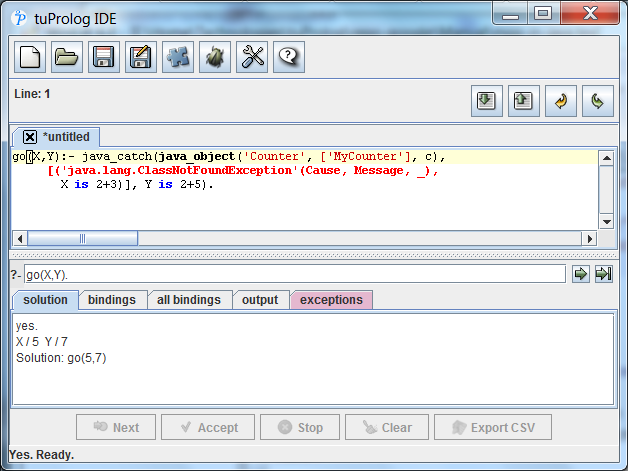
\includegraphics[width=7cm]{images/exceptions1a}
  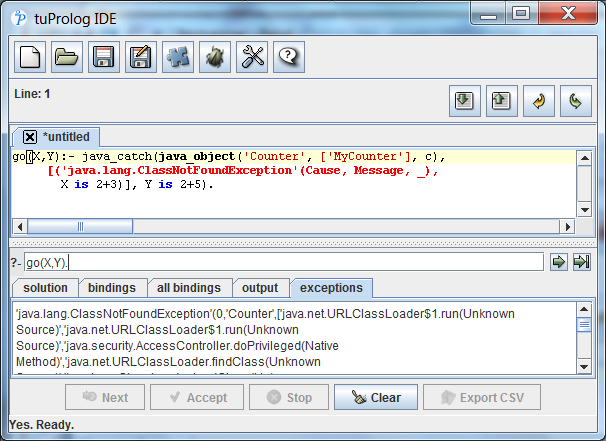
\includegraphics[width=7cm]{images/exceptions1b}
  \caption{Catching the Java exceptions of Example 1 in the \tuprolog{} GUI.
  \textit{Top:} the solutions tab.
  \textit{Bottom:} details of the exception in the exception tab (see the \texttt{Cause} variable bound to \texttt{0} and the \texttt{Msg} variable bound to \texttt{'Counter'}; the other details map onto the anonymous variable \texttt{\_}). }\label{fig:exceptions1}
\end{figure}


\medskip\noindent
\textit{\textbf{Example 2:} execution must fail if an exception is raised during the execution of a goal and no matching \texttt{java\_catch/3} is found.}
\begin{verbatim}
 ?- java_catch(java_object('Counter', ['MyCounter'], c),
      [('java.lang.Exception'(Cause, Message, _), true)], true)).
\end{verbatim}

Answer: \texttt{ no.}

\noindent In the \tuprolog{} GUI, a failed exception not only results into a "No" answer as in other Prolog systems (that answer is shown in the status bar at the bottom of the window: it also causes the \textit{halt} message to appear in the Solutions tab (Figure \ref{fig:exceptions2}).

\begin{figure}
  \centering
  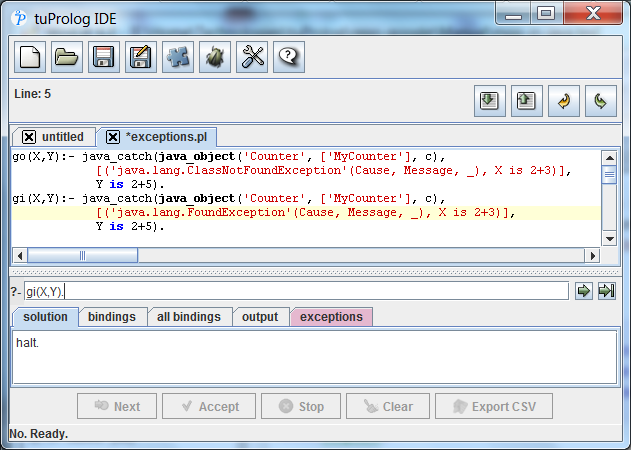
\includegraphics[width=7cm]{images/exceptions2}
  \caption{A failed exception in the \tuprolog{} GUI: the \texttt{No} answer in the status bar and the \textit{halt} message in the Solutions tab.}
  \label{fig:exceptions2}
\end{figure}


\medskip\noindent
\textit{\textbf{Example 3:} \texttt{java\_catch/3} must fail if the handler is false.}
\begin{verbatim}
 ?- java_catch(java_object('Counter', ['MyCounter'], c),
      [('java.lang.Exception'(Cause, Message, _), false)], true)).
\end{verbatim}

Answer: \texttt{ no.}

\medskip\noindent
\textit{\textbf{Example 4:} \texttt{java\_catch/3} must fail also if an exception is raised during the execution of the handler.}
\begin{verbatim}
 ?- java_catch(java_object('Counter', ['MyCounter'], c),
      [('java.lang.ClassNotFoundException'(Cause, Message, _),
        java_object('Counter', ['MyCounter'], c))], true).
\end{verbatim}

Answer: \texttt{ no.}

\medskip\noindent
\textit{\textbf{Example 5:} the \textit{\texttt{Finally}} must be executed also in case of success of the goal.}
\begin{verbatim}
 ?- java_catch(java_object('java.util.ArrayList', [], l),
       [E, true], X is 2+3).
\end{verbatim}

Answer: \texttt{ yes.}

Substitutions: \texttt{X/5}.

\medskip\noindent
\textit{\textbf{Example 6:} the \textit{\texttt{Handler}} to be executed must be the proper one among those available in the handlers' list.}
\begin{verbatim}
 ?- java_catch(java_object('Counter', ['MyCounter'], c),
     [('java.lang.Exception'(Cause, Message, _), X is 2+3),
      ('java.lang.ClassNotFoundException'(Cause, Message, _), Y is 3+5)],
      true).
\end{verbatim}

Answer: \texttt{ yes.}

Substitutions: \texttt{Cause/0}, \texttt{Message/'Counter'}, \texttt{Y/8}.

%-----------------------------------------------------------------------
\newpage
\section{Using Prolog from Java: \textit{the Java API}}
\label{sec:java-api}
%-----------------------------------------------------------------------

The \tuprolog{} Java API provides a complete support for exploiting Prolog engines from Java: its only requirement is the presence of \texttt{tuprolog.jar} (or the more complete \texttt{2p.jar}) in the Java project's class path.
The API defines a namespace (\texttt{alice.tuprolog}) and classes to enable the definition in Java of suitable objects representing Prolog entities (terms, atoms, lists, variables, numbers, etc, but also Prolog engines, libraries and theories), and use them to submit queries and get the results back in Java, thus effectively supporting multi-paradigm, multi-language programming.

%-----------------------------
\subsection{A Taxonomy of Prolog types in Java}
\label{ssec:java-api-types}
%-----------------------------

Prolog types are mapped onto suitable Java classes, organized into the taxonomy shown in Figure \ref{fig:term-taxonomy} and summarized in Table \ref{tab:prolog-java-type-mapping} on page \pageref{tab:prolog-java-type-mapping}.

\begin{figure}[b]
    \setlength{\unitlength}{1mm}
    \begin{picture}(80,27){\scriptsize
        \put(30,11){\framebox(13,5){Term}}
        %
        \put(50, 3){\framebox(13,5){Struct}}
        \put(50,11){\framebox(13,5){Number}}
        \put(50,19){\framebox(13,5){Var}}
        %
        \put(70, 3){\framebox(13,5){Int}}
        \put(90, 3){\framebox(13,5){Long}}
        \put(70,19){\framebox(13,5){Float}}
        \put(90,19){\framebox(13,5){Double}}

        \put(43,13.5){\line(1,0){6.5}}
        \put(63,13.5){\line(1,0){24}}
        %
        \put(67,21){\line(1,0){3}}
        \put(67,5.5){\line(1,0){3}}
        \put(67,21){\line(0,-1){15.5}}
        %
        \put(47,21){\line(1,0){3}}
        \put(47,5.5){\line(1,0){3}}
        \put(47,21){\line(0,-1){15.5}}
        %
        \put(87,21){\line(1,0){3}}
        \put(87,5.5){\line(1,0){3}}
        \put(87,21){\line(0,-1){15.5}}
    }
    \end{picture}
    \caption{Prolog entities as a taxonomy of Java classes.}
    \label{fig:term-taxonomy}
\end{figure}

\texttt{Term} is the root abstract class, providing common services such as term unification, term parsing, term copying, etc.; its subclasses distinguish among untyped terms (structures), numbers, and variables.

\texttt{Struct} objects are characterized by a functor name (a Java string) and
a list of arguments, which are \texttt{Term}s themselves and can be
individually retrieved via the \texttt{getTerm} method.

Atoms are a special case of \texttt{Struct} with no arguments; among these, the \texttt{true} and \texttt{false} atom constants are used to represent the Java boolean values.
Atoms are also used to map Java \texttt{char}s and strings: when converted back to Java, however, atoms are always mapped into Java \texttt{String}s.

Prolog lists are another special case of \texttt{Struct}, built from either
two \texttt{Term}s (the list head and tail) or an array of \texttt{Term}s; by
convention, the default constructor builds the empty list.

The \texttt{Number} subtree includes classes for numeric types, and offers methods such as \texttt{intValue}, \texttt{longValue}, etc. to retrieve the number value as the corresponding primitive Java value.
As discussed above, in the Prolog-to-Java direction, Prolog integers are always mapped onto \texttt{Int} instances and Prolog reals onto \texttt{Double} instances, while in the Java-to-Prolog direction any of the numeric Java types are accepted (including \texttt{short}, \texttt{byte} and \texttt{float}) for mapping onto Prolog numbers.
In particular, Java \texttt{int} and \texttt{long} values are mapped onto suitable \texttt{Int} and \texttt{Long} instances of the \tuprolog{} taxonomy, respectively, while \texttt{byte} and \texttt{short} Java types are mapped into \texttt{Int} instances.
Please note that to avoid possible name clashes between \tuprolog{} types and Java wrapper classes (e.g. \texttt{alice.tuprolog.Long} and \texttt{java.lang.Long}), it is often necessary to use the fully qualified class name to denote \tuprolog{} numeric classes.

\texttt{Var} represents Prolog variables, built from a Java string representing the variable name: as prescribed by the Prolog rules, the name must start either with a capital letter, or with an underscore.
The default constructor builds the anonymous Prolog variable \texttt{\_}, mapped onto the Java \texttt{null} value.

Table \ref{tab:creating-prolog-terms-in-java} on page \pageref{tab:creating-prolog-terms-in-java} shows how to manipulate Prolog entities (variables, terms, structures, lists, atoms..) from a Java program: variable creation (lines 1 and 10), list construction (lines 2--4), term construction for \texttt{p(a,5)} and \texttt{p(X,Y)} (lines 5--6), and term unification (lines 7--14) (the latter requires a Prolog engine as a mediator, to handle execution contexts and inner variables).

It is worth noting that, in general, two different \texttt{Var} objects with the same Java name \textit{do not} refer to the same Prolog variable, unless they occur in the same term.
So, multiple occurrences of \texttt{new Var("Y")} outside the same term refer to two distinct variables, as if they were renamed \texttt{Y1} and \texttt{Y2}.
%
To refer to the same Prolog variable twice, just use the same Java identifier (see \texttt{varY} in lines 1, 3, 12) instead of creating a new variable.

The only exception is the case when the homonymous variables occur in the same term, as in the \texttt{q(Y,Y)} term in line 15: then, they will refer to the same variable, \textit{but only after the term has been resolved}.
In fact, new terms are always built in an `unresolved' form, that does not analyze the term variables: the proof is the \textit{\texttt{false}} output of line 16.
Variables are taken into consideration later, when the term is either explicitly resolved via \texttt{resolveTerm} (line 17), or is involved in a \texttt{match} or \texttt{unify}\footnote{\texttt{q(Y,Y)} is unified here with the Prolog anonymous variable, so success is granted.} operation with another term (lines 18-19), as proved by the \textit{\texttt{true}} output of line 20.

\begin{table}[h]
    \small
    \begin{center}{\tt
    \begin{tabular}{p{13cm}}\hline\\
    \mbox{~~~}import alice.tuprolog.*;\\
    \mbox{~~~}\ldots\\
    \mbox{1~~}Var varX = new Var("X"), varY = new Var("Y"); \\
    \mbox{2~~}Struct atomP = new Struct("p");\\
    \mbox{3~~}Struct list = new Struct(atomP, varY);~~~~~~~\textit{// should be [p|Y]}\\
    \mbox{4~~}System.out.println(list);~~~~~~~~~~~~~~\textit{// prints the list [p|Y]}\\
    \mbox{5~~}Struct fact = new Struct("p", new Struct("a"), new Int(5));\\
    \mbox{6~~}Struct goal = new Struct("p", varX, new Var("Z"));\\
    \mbox{7~~}Prolog engine = new Prolog();\\
    \mbox{8~~}boolean res = goal.unify(engine,fact);~~~~~\textit{// should be X/a, Y/5}\\
    \mbox{9~~}System.out.println(goal);~~~~~\textit{// prints the unified term p(a,5)}\\
    \mbox{10~}System.out.println(varX);~~~~~\textit{// prints the variable binding X/a}\\
    \mbox{11~}Var varW = new Var("W");\\
    \mbox{12~}res = varW.unify(engine,varY);~~~~~~~~~~~~~~~~~~\textit{// should be Z=Y}\\
    \mbox{13~}System.out.println(varY);~~\textit{// prints just Y, since it is unbound}\\
    \mbox{14~}System.out.println(varW);~~\textit{// prints the variable binding W / Y}\\
    \mbox{15~}Struct st = Struct("q", new Var("Y"), new Var("Y"));~\textit{// unresolved}\\
    \mbox{16~}System.out.println(st.getArg(0)==st.getArg(1));~~\textit{// prints false}\\
    \mbox{17~}st.resolveTerm();~~~~~~~~~~~~~~~~~~~\textit{// now the term is resolved}\\
    \mbox{18~}~~\textit{alternatively:} res = st.match(new Struct());\\
    \mbox{19~}~~\textit{alternatively:} res = st.unify(engine, new Struct());\\
    \mbox{20~}System.out.println(st.getArg(0)==st.getArg(1));~~\textit{// prints true}\\
    \\\hline
    \end{tabular}}
    \end{center}
    \caption{Manipulating Prolog entities from Java.}
    \label{tab:creating-prolog-terms-in-java}
\end{table}

\subsubsection{Further notes about \texttt{Term}s}

The \texttt{Term} class is the home of several general-purpose services, used throughout \tuprolog{}; in particular:

\begin{itemize}
\item the static \texttt{parse} and \texttt{createTerm} methods provides a quick way  to get a term from its string representation;

\item the \texttt{match} and \texttt{unify} methods respectively check for term matching (but performing no actual unification) and unify the given term with the provided one; as anticipated above, the latter requires a \texttt{Prolog} argument, to be used as a mediator during (nested) unification;
    Instead, the matching test is performed outside any demonstration context.

\item the \texttt{equals} method compares terms with the same semantics of the method \texttt{isEqual}, which follows the Prolog comparison semantics.

\item the \texttt{getTerm} method returns the referred term, following variable bindings---that is, if the target term is a bound variable, the term bound to the variable (not the variable itself) is returned.
\end{itemize}


%-----------------------------
\subsection{Prolog engines, theories and libraries}
\label{ssec:java-api-engine-solveinfo}
%-----------------------------

The \tuprolog{} engine is made accessible in Java via the \texttt{Prolog} class: so, adding intelligence to a Java program is as easy as creating \texttt{Prolog} instance(s), configure it (them) as needed, and perform the desired queries. Query results are expressed as an instance of the \texttt{SolveInfo} helper class.
Table \ref{tab:engine-interface} reports the public interface of these classes.

\begin{table}
    \renewcommand\arraystretch{1}
    \begin{center}{\tt
    \begin{tabular}{p{14cm}}\hline\\
    public class Prolog implements Serializable \{\\
    ~~\ldots\\
    ~~public void setTheory(Theory t) throws InvalidTheoryException \{\ldots\}\\
    ~~public void addTheory(Theory t) throws InvalidTheoryException \{\ldots\}\\
    ~~public Theory getTheory() \{\ldots\}\\
    ~~public Library loadLibrary(String name)\\
    ~~~~~~~~~~~~~~~~~~~~~~~~~~~~~~~~~throws InvalidLibraryException \{\ldots\}\\
    ~~public void~unloadLibrary(String name)\\
    ~~~~~~~~~~~~~~~~~~~~~~~~~~~~~~~~~throws InvalidLibraryException \{\ldots\}\\
    ~~public Library getLibrary(String name) \{\ldots\}\\
    ~~public SolveInfo solve(Term goal) \{\ldots\}\\
    ~~public SolveInfo solve(String goalAsString)\\
    ~~~~~~~~~~~~~~~~~~~~~~~~~~~~~~throws MalformedGoalException \{\ldots\}\\
    ~~public boolean hasOpenAlternatives() \{\ldots\}\\
    ~~public SolveInfo solveNext()~throws NoMoreSolutionException \{\ldots\}\\
    ~~public boolean isHalted() \{\ldots\}\\
    \}\\
    \\\hline\\
    public class SolveInfo implements Serializable \{\\
    ~~public boolean isSuccess() \{\ldots\}\\
    ~~public Substitution getSubstitution()\\
    ~~~~~~~~~~~~~~~~~~~~~~~~~~~~~~throws NoSolutionException \{\ldots\}\\
    ~~public Term getTerm() throws UnknownVarException \{\ldots\}\\
    ~~public Term  getSolution() throws NoSolutionException \{\ldots\}\\
    \}\\
    \\\hline
    \end{tabular}}
    \end{center}
    %
    \caption{Classes for interacting with \tuprolog{} engines.}
    \label{tab:engine-interface}
\end{table}

A Prolog engine is built by one of \texttt{Prolog} constructors: the default constructor builds a default engine, with the default set of \tuprolog{} libraries loaded, and no user theory. In most cases, this is all you need to bring the power of Logic programming to Java.
%
However, libraries can be loaded and unloaded dynamically at any time after the engine creation, via the \texttt{loadLibrary} and \texttt{unloadLibrary} methods: their argument is the name of the library. If the library is invalid, an exception is raised.
%
A reference to a loaded library can be obtained via the \texttt{getLibrary} method, which returns a reference to the abstract \texttt{Library} class.
%
Such a reference can be used to operate on the library, as discussed below.

The user theory can either be set from scratch via the \texttt{setTheory} method, which overwrites any previous theory, or be built incrementally, adding new clauses to the existing theory via the \texttt{addTheory} method: both take a \texttt{Theory} as their argument. This theory can be built in several ways---from an input stream, from a string, or from a clause list (represented as a \texttt{Struct} object---see the example in Table \ref{tab:java-api-example-clauselist} on page \pageref{tab:java-api-example-clauselist} for details).
%
The current theory can be retrieved via the \texttt{getTheory} method.

Goal resolution is handled via three methods: \texttt{solve}, \texttt{solveNext}, and
\texttt{hasOpenAlternatives}.
%
\texttt{solve} and \texttt{solveNext} take as their argument a \texttt{Struct} representing the goal, and return a \texttt{SolveInfo} which encapsulates the result information (success or failure, solution, variable bindings, etc).
%
An overloaded version of \texttt{solve} takes a string argument representing the text of the goal, embedding its parsing.
%
Both \texttt{solve} and \texttt{solveNext} raise the proper exceptions when needed.


\subsubsection{Further notes about \texttt{Prolog} engines}

The \texttt{Prolog} class is the home of \tuprolog{} engines, so some further information is opportune about its behavior in particular contexts:

\begin{itemize}
\item engines support natively some \emph{directives}, that can be defined by means of the \texttt{:-/1} predicate in theory specification.
    Directives are used to specify properties of clauses and engines (\texttt{solve/1}, \texttt{initialization/1}, \texttt{set\_prolog\_flag/1}, \texttt{load\_library/1}, \texttt{include/1}), format and syntax of read-terms (\texttt{op/3}, \texttt{char\_conversion/2}).

\item engines also support the dynamic definition and management of \emph{flags} (or property), used to describe some aspects of libraries and their built-ins.
    A flag is identified by a name (an alphanumeric atom), a list of possible values, a default value and a boolean value specifying if the flag value can be modified.

\item engines are thread-safe.

\item engines have no (static) dependencies with each other, can be created  independently on the same Java virtual machine, are very lightweight, and can be serialized.
    This is true also for engines with the standard libraries pre-loaded: obviously, if other libraries are loaded, these must be serializable, too, for the engine to remain serializable.
\end{itemize}

%-------------------------------------------------------
\subsection{Examples}
\label{ssec:java-api-examples}
%-------------------------------------------------------

For the sake of concreteness, some examples of use of the \tuprolog{} Java API are now discussed.

%--------------
\subsubsection{Appending lists}
%--------------

\begin{table}
\textit{Basic version:}
{\small{
\begin{verbatim}
    import alice.tuprolog.*;

    public class Example1 {
        public static void main(String[] args) throws Exception {
            Prolog engine = new Prolog();
            SolveInfo info = engine.solve("append([1],[2,3],X).");
            System.out.println(info.getSolution());
        }
    }
\end{verbatim}
}}
\textit{Variant:}
{\small{
\begin{verbatim}
    import alice.tuprolog.*;

    public class Example2 {
        public static void main(String[] args) throws Exception {
            Prolog engine = new Prolog();
            SolveInfo info = engine.solve("append(X,Y,[1,2]).");
            while (info.isSuccess()) {
                System.out.println("solution: " + info.getSolution() +
                                   " - bindings: " + info);
                if (engine.hasOpenAlternatives()) {
                    info = engine.solveNext();
                } else {
                    break;
                }
            }
        }
    }
\end{verbatim}
}}
\caption{The list appending example.}
\label{tab:java-api-example1}
\end{table}

In this first example (see Table \ref{tab:java-api-example1}, \textit{top}), a \tuprolog{} engine is asked to solve a trivial list append goal, provided in textual form.\footnote{The \texttt{append/3} predicate is included in BasicLibrary, which is part of the engine default configuration.}
%
The program must be compiled and executed normally, taking care of including the \tuprolog{} JAR in the classpath:

\texttt{javac -cp tuprolog.jar;. Example1.java}\\
\texttt{\mbox{~~~}java~ -cp tuprolog.jar;. Example1}

\noindent The string \texttt{append([1],[2,3],[1,2,3])} should be displayed.

\medskip

\noindent Table \ref{tab:java-api-example1}, \textit{bottom} shows a variant where all the solutions are displayed, with their variable bindings. The output should be as follows:

\begin{verbatim}
solution: append([],[1,2],[1,2]) - bindings: X/[]    Y/[1,2]
solution: append([1],[2],[1,2])  - bindings: X/[1]   Y/[2]
solution: append([1,2],[],[1,2]) - bindings: X/[1,2] Y/[]
\end{verbatim}


%--------------
\subsubsection{Exploiting a theory from clause list}
%--------------

\begin{table}
{\small{
\begin{verbatim}
import alice.tuprolog.*;

public class Main {

  public static void main(String[] args) throws InvalidTheoryException,
      MalformedGoalException, NoSolutionException, NoMoreSolutionException {

      Struct clause1 = new Struct(":-", new Struct("p",new Var("X")),
                                        new Struct("q",new Var("X")));
      Struct clause2 = new Struct(":-", new Struct("q",new Int(0)),
                                        new Struct("true"));
      System.out.println(clause1 + " is a clause? " + clause1.isClause());
      System.out.println(clause2 + " is a clause? " + clause2.isClause());

      Prolog engine = new Prolog();
      Struct clauseList = new Struct(clause1,
                                     new Struct(clause2, new Struct()));
      System.out.println(clauseList + " is a list? " + clauseList.isList());

      Theory t = new Theory(clauseList);
      engine.addTheory(t);
      SolveInfo info = engine.solve("p(X).");

      while (info.isSuccess()) { % taken from the previous example
        System.out.println("solution: " + info.getSolution() +
                           " - bindings: " + info);
        if (engine.hasOpenAlternatives()) {
          info = engine.solveNext();
        } else {
          break;
        }
      }

    }
}
\end{verbatim}
}}
\caption{Building a theory ``by hand'' from a clause list.}
\label{tab:java-api-example-clauselist}
\end{table}

In this example (see Table \ref{tab:java-api-example-clauselist}), a \tuprolog{} theory is built from a clause list.
As in any standard Prolog, a \tuprolog{} clause is just a structure whose functor is \texttt{`:-'}/2. In their turn, facts are expressed as clauses whose body is the atom \texttt{true}, which can be built as a new \texttt{Struct("true")} (the same holds for the atom \texttt{false}, of course). Accordingly, \texttt{clause1} and \texttt{clause2} represent the \texttt{p(X):-q(X).} and \texttt{q(0):-true.} clauses, respectively.
In order to make the example more explanatory, a couple of print statements have been added that check whether \texttt{clause1} and \texttt{clause2} are actually valid clauses, via the \texttt{Term.isClause} method.

A clause list is just what it name says: a prolog list whose terms are clauses. Since lists are just \texttt{Struct} instances built from a term and another list (possibly the empty list built by the default \texttt{Struct} constructor), the desired clause list is built by creating a \texttt{Struct} having \texttt{clause1} as its first argument, and another list as its second argument: the latter is built by creating a \texttt{Struct} having \texttt{clause2} as its first argument, and the empty list as its second argument. Again, a print statement has been added to show that the \texttt{clauseList} term is actually a valid list.
The clause list is then used to construct the new theory, as required.

In order to make the example more complete, the engine is finally asked to solve the \texttt{p(X).} query, which obviously has \texttt{p(0)} as its only solution; the same exploration cycle presented in Table \ref{tab:java-api-example1} is re-used for this purpose.

%--------------
\subsubsection{A console-based Prolog interpreter}
%--------------

\begin{table}
    \small
    \begin{center}{\tt
    \begin{tabular}{p{14cm}}\hline\\
    import alice.tuprolog.*;\\
    import java.io.*;\\
    \\
    public class ConsoleInterpreter  \{\\
    ~public static void main (String args[]) throws Exception \{\\
    ~~Prolog engine=new Prolog();\\
    ~~if (args.length>0)\\
    ~~~~~~engine.setTheory(new Theory(new FileInputStream(args[0])));\\
    ~~BufferedReader stdin =\\
    ~~~~~~new BufferedReader(new InputStreamReader(System.in));\\
    ~~while (true) \{ \textit{~~~~// interpreter main loop} \\
    ~~~String goal;\\
    ~~~do \{ System.out.print("?- "); goal=stdin.readLine();\\
    ~~~\} while (goal.equals(""));\\
    ~~~try \{\\
    ~~~~SolveInfo info = engine.solve(goal);\\
    ~~~~if (engine.isHalted()) break;\\
    ~~~~else if (!info.isSuccess()) System.out.println("no.");\\
    ~~~~else if (!engine.hasOpenAlternatives()) \{\\
    ~~~~~~System.out.println(info);\\
    ~~~~\} else \{ \textit{// main case}\\
    ~~~~~~System.out.println(info + " ?");\\
    ~~~~~~String answer = stdin.readLine();\\
    ~~~~~~while (answer.equals(";") \&\& engine.hasOpenAlternatives())
    \{\\
    ~~~~~~~~info = engine.solveNext();\\
    ~~~~~~~~if (!info.isSuccess()) \{ System.out.println("no."); break; \}\\
    ~~~~~~~~else \{\\
    ~~~~~~~~~~~~~~~System.out.println(info + " ?");\\
    ~~~~~~~~~~~~~~~answer = stdin.readLine();\\
    ~~~~~~~~\} \textit{// endif}\\
    ~~~~~~\} \textit{// endwhile}\\
    ~~~~~~if (answer.equals(";") \&\& !engine.hasOpenAlternatives())\\
    ~~~~~~~~~~System.out.println("no.");\\
    ~~~~\} \textit{// end main case}\\
    ~~~\} catch (MalformedGoalException ex) \{\\
    ~~~~~~~~~~System.err.println("syntax error.");\\
    ~~~\} \textit{// end try}\\
    ~~\} \textit{// end main loop}\\
    ~~if (args.length>1) \{\\
    ~~~Theory curTh = engine.getTheory(); \textit{// save current theory to file}\\
    ~~~new
    FileOutputStream(args[1]).write(curTh.toString().getBytes());\\
    ~~\}\\
    ~\}\\
    \}\\
    \\\hline
    \end{tabular}}
    \end{center}
    \caption{A simple console-based Prolog interpreter.}
    \label{tab:console-sample}
\end{table}

As a final example, Table \ref{tab:console-sample} shows a console-based Prolog interpreter: first a \tuprolog{} engine is created and initialized with a theory built from a text file (whose name is taken from the command line), then a classic read/solve loop is started.

For each goal read from the standard input, the \texttt{solve} method is invoked: if multiple solutions exist, the \texttt{solveNext} makes it possible to explore the open alternatives.
%
The loop ends when the \texttt{halt} predicate is typed in: the current theory is then saved to file (if any has been specified).
Figure \ref{fig:console-interpreter} shows a sample session with this interpreter.

\begin{figure}
  \centering
  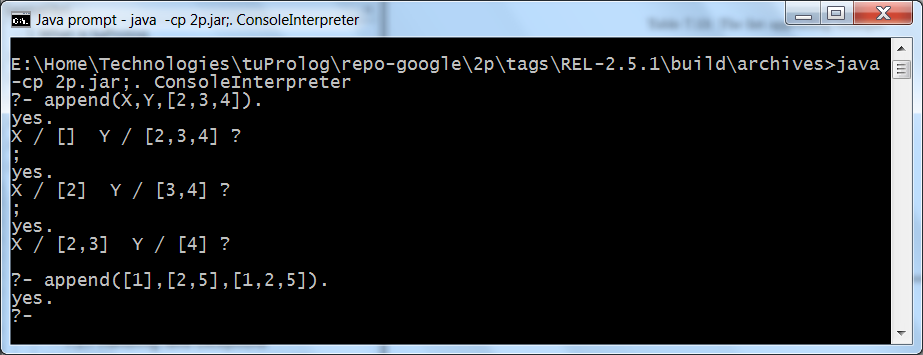
\includegraphics[width=12cm]{images/console-interpreter}
  \caption{A sample session with the Console-based Interpreter.}
  \label{fig:console-interpreter}
\end{figure}


%-----------------------------------------------------------------------
\subsection{Support to relative paths in consulting Prolog sub-files}
\label{ssec:relative-paths-consulting-subfiles-in-java-project}
%-----------------------------------------------------------------------

When developing a Java project that needs to load some Prolog theory, the typical Java statement to do so is:

\begin{verbatim}
   Theory theory = new Theory(new FileInputStream("test.pl"));
\end{verbatim}

\noindent In this way, however, only the files on the root folder of the Java project can be found and located: files in any other folder require either an absolute path, or a relative path starting from the project base folder (like \texttt{src/prolog-folder/subfile.pl}).

This is quite uncomfortable, as it can easily lead either to prevent project relocation (if absolute paths are used) or  obstruct the otherwise-natural idea to put all the Prolog files in a suitable \texttt{prolog-files} subfolder (due to the need to refer to the project base folder, which would call for relative paths like \texttt{src/prolog-folder/subfile.pl}).

To overcome these limitations, \tuprolog{} 2.7 improves the default behaviour of the \texttt{consult} predicate by allowing
paths to be specified that are \textit{relative to the folder of the Prolog file which is doing the call}.

In this way, Prolog files can be placed in a suitable \texttt{prolog-files} subfolder, and properly referenced by other files in upper folders easily and directly. For instance, if the Java project structure is something like:

\begin{verbatim}
- src
- prolog-folder/
- main.pl
- java-folder/
...
\end{verbatim}

\noindent the \texttt{main.pl} file can now include \texttt{subfile.pl} in the \texttt{prolog-folder} subfolder via a simple \texttt{consult('subfile.pl')} command.
%
In order to exploit this mechanism from Java, statements like the previous:

\begin{verbatim}
   Theory theory = new Theory(new FileInputStream("test.pl"));
\end{verbatim}

\noindent must be replaced by:

\begin{verbatim}
   Theory theory = new Theory(":-consult('test.pl').");
\end{verbatim}
 
\noindent In this way, the file location process is delegated to the \tuprolog{} engine instead of depending on Java's built-in \texttt{FileInputStream} mechanism.

As an aside, this improvement also covers the \tuprolog{} IDE, enabling the sub-inclusions of Prolog files from other Prolog files in different folders even in the interactive work sessions.
So, for instance, after consulting from the IDE a prolog file located in \texttt{someOtherFolder} (that is, a folder other than the current one), you can use \texttt{consult(someOtherFile)} command to load a file from the current folder.


%-----------------------------------------------------------------------
\subsection{Registering object bindings}
\label{ssec:register(Java)}
%-----------------------------------------------------------------------

The \texttt{register} function, already discussed in Section \ref{sssec:register(prolog)} on page \pageref{sssec:register(prolog)} for what concerns the Prolog side, is also available on the Java side, where its `global' effect is more natural and coherent with the imperative paradigm than it is on the Prolog side.

Its purpose is to permanently associate an existing Java object \texttt{\textit{obj}} to a Prolog identifier \texttt{\textit{ObjectRef}}, as follows:\\

\texttt{boolean register(Struct \textit{ObjectRef}, Object \textit{obj})\\
    \mbox{~~~~~~~~~~~}throws InvalidObjectIdException;}\\

\noindent where \texttt{\textit{ObjectRef}} is a ground term (otherwise an \texttt{InvalidObjectIdException} exception is raised) representing the Java object
\texttt{\textit{obj}} in the context of \texttt{JavaLibrary}'s predicates.
The function returns \texttt{false} if that object is already registered under a different \texttt{\textit{ObjectRef}}.

As an example, let us suppose that we want to permanently bind the Prolog atom \texttt{stdout} to the Java (static) object \texttt{System.out}, so that Java-based printing can be done from the Prolog side without having to retrieve and re-bind the \texttt{out} object every time, as we did in Table \ref{tab:javalibrary-counter-example} on page \pageref{tab:javalibrary-counter-example} (reported again below for convenience):

\begin{verbatim}
  class('java.lang.System') . out <- get(Out),
  Out <- println(...),
\end{verbatim}

\noindent To bind \texttt{System.out} permanently to \texttt{stdout} (within the scope of the \tuprolog{} engine \texttt{engine}), we can register it as follows:

{\small
\begin{verbatim}
  Prolog engine = new Prolog();
  Library lib = engine.getLibrary("alice.tuprolog.lib.JavaLibrary");
  ((JavaLibrary)lib).register(new Struct("stdout"), System.out);
\end{verbatim}}

\noindent An explicit downcast to \texttt{JavaLibrary} is needed to convert the returned reference type \texttt{Library}, since \texttt{register} is defined in \texttt{JavaLibrary} only.
%
Now, a Prolog theory loaded into this \texttt{engine} can contain a phrase like:
%
\begin{verbatim}
  stdout <- println('What a nice message!')
\end{verbatim}
%
which uses \texttt{stdout} directly as a target for the \texttt{println} method.

A small yet complete sample program is shown in Table \ref{tab:registering-stdout-example}, where the theory loaded into the \texttt{engine} prints the standard greetings message.

\begin{table}[h]
{\small
\begin{verbatim}
  import alice.tuprolog.*;
  import alice.tuprolog.lib.*;

  public class StdoutExample {
    public static void main(String[] args) throws Exception {
    Prolog engine = new Prolog();
    Library lib = engine.getLibrary("alice.tuprolog.lib.JavaLibrary");
    ((JavaLibrary)lib).register(new Struct("stdout"), System.out);
    engine.setTheory(new Theory(
        ":-solve(go). \n go:- stdout <- println('hello!')."));
    }
 }
\end{verbatim}}
\caption{A program registering \texttt{stdout} for \texttt{System.out}. As an alternative to \texttt{getLibrary}, \texttt{loadLibrary} could have been used---if the library is already loaded, its behavior is identical to \texttt{getLibrary}'s.
%
Also, the fully qualified class name \texttt{"alice.tuprolog.lib.JavaLibrary"} is needed in \texttt{getLibrary} only because \texttt{JavaLibrary} does \textit{not} define a short library name (see Section \ref{ssec:library-name} for details): otherwise, the shorter name could have been used.}
\label{tab:registering-stdout-example}
\end{table}

%-------------------------------------------------------
\subsection{Capturing the Prolog output in Java}
\label{ssec:capturing-output}
%-------------------------------------------------------

If a \tuprolog{} engine is used in a Java application, the output performed by Prolog \texttt{write} predicates (more generally, of any predicate writing on the Prolog console) is not available in Java: printed messages are not captured, nor are they retrievable by any of the \tuprolog{} Java API methods.
%
The only way to `capture' somehow the output of the Prolog engine is to write it to a file or store it in a Prolog term---just two variants of the same inconvenience.

Yet, this feature can be added in a non-intrusive way, thanks to \tuprolog{}'s extensible architecture, by simply overriding the \texttt{onOutput} method used internally by the engine to handle the write requests.\footnote{This approach was originally suggested by Josh Guzman in the \tuprolog{} users' forum.}
All is needed is to redefine this method so as to capture the output message and store it conveniently---for instance, into a suitable \texttt{String} of the Java application (here, \texttt{finalResult}), as follows:

\begin{verbatim}
  engine.addOutputListener(new OutputListener() {
    @Override
    public void onOutput(OutputEvent e) {
      finalResult += e.getMsg();
    }
  });
\end{verbatim}

\noindent This elegant approach does not modify the \tuprolog{} code in any way: it just adds listener to an existing event, extending the service non-intrusively.
%
A full example of this technique is reported in Table
\ref{tab:capturing-output-complete} on page \pageref{tab:capturing-output-complete}, together with the corresponding build process and execution.

\begin{table}[h]
{\small
\begin{verbatim}
  import alice.tuprolog.*;
  import alice.tuprolog.lib.*;
  import alice.tuprolog.event.*;

  public class OnOutputExample {
    static String finalResult = "";
    public static void main(String[] args) throws Exception {
      Prolog engine = new Prolog();
      engine.addOutputListener(new OutputListener() {
          @Override
          public void onOutput(OutputEvent e) {
            finalResult += e.getMsg();
          }
      });
      Term goal = Term.createTerm("write('Hello world!')");
      SolveInfo res = engine.solve(goal);
      res = engine.solve("write('Hello everybody!'), nl.");
      System.out.println("OUTPUT: " + finalResult);
    }
  }
\end{verbatim}}
\centering
  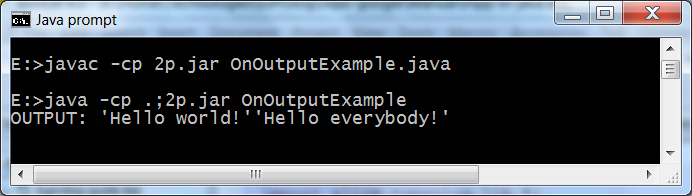
\includegraphics[width=12cm]{images/onOutput}
\caption{Capturing the Prolog output from Java: a complete example.}
\label{tab:capturing-output-complete}
\end{table}

%-----------------------------------------------------------------------
\section{Augmenting Prolog via Java:\\developing new libraries}
\label{sec:howto-develop-libraries}
%-----------------------------------------------------------------------

So far, the two first dimensions of \tuprolog{}'s support to multi-paradigm, multi-language programming have been explored, that enable a language (and the corresponding paradigm) to be used from the other.
The two further dimensions concerns \textit{augmenting} the language instead---that is, exploiting a language (and a paradigm) to increase the other.

In this section the focus is on augmenting Prolog from Java, exploiting the latter\footnote{%
 Other languages may be used indirectly, via JNI (JavaNative Interface}
to increase the first by developing new \tuprolog{} libraries; the next Section (\ref{sec:p@j}) will focus on the opposite direction, exploiting Prolog to augment Java via the so-called \textit{P@J} framework.

Moreover, although \tuprolog{} libraries are expressed in Java, they are not required to
be fully implemented in this language.
%
In fact, Java-only libraries are the simplest case, but hybrid Java + Prolog libraries are also possible, where a Prolog theory is embedded into a Java string so that the
two parts cooperate to define the overall library behavior.
This opens further interesting perspectives, that will be discussed below.

%---------------------------------------------------------------
\subsection{Syntactic conventions}
\label{ssec:library-syntax}
%---------------------------------------------------------------
Each library must extend the base abstract class \texttt{alice.tuprolog.Library} and define new \textit{predicates} and/or \textit{evaluable functors} and/or \textit{directives} in the form of methods, following a simple signature convention.

\noindent Predicates must adhere to the signature:\\

{\small\tt
%    public boolean <\textit{pred name}>\_<\textit{N}>(\textit{T1} arg1, \textit{T2} arg2, ...,\textit{Tn} argN)
    public boolean <\textit{pred name}>\_<\textit{N}>(\\
    \mbox{~~~~~~~~~~~~}<?~extends~Term> arg1, ..., <?~extends~Term> argN)
}\\

\noindent while evaluable functors must follow the form:\\

{\small\tt
%    public Term <\textit{eval funct name}>\_<\textit{N}>(\textit{T1} arg1, \textit{T2} arg2, ...,\textit{Tn} argN)
    public Term <\textit{eval funct name}>\_<\textit{N}>(\\
    \mbox{~~~~~~~~~~~~}<?~extends~Term> arg1, ..., <?~extends~Term> argN)
}\\

\noindent and directives must be provided with the signature:\\

{\small\tt
%    public void <\textit{dir name}>\_<\textit{N}>(\textit{T1} arg1, \textit{T2} arg2, ..., \textit{Tn} argN)
    public void <\textit{dir name}>\_<\textit{N}>(\\
    \mbox{~~~~~~~~~~~~}<?~extends~Term> arg1, ..., <?~extends~Term> argN)
}\\

\noindent where \textit{arg1}, ... \textit{argN} are \texttt{Term}s\footnote{%
 Please refer to Table \ref{fig:term-taxonomy} on page \pageref{fig:term-taxonomy} for the full Term taxonomy.}
that represent the actual arguments passed to the predicate (functor, directive).

\begin{table}
    \begin{center}{\small\tt
    \begin{tabular}{p{12cm}}
     \hline\\
    import alice.tuprolog.*;\\
    public class TestLibrary extends Library \{\\
    \\
    ~~\textit{// functor sum(A,B)}\\
    ~~public Term sum\_2(Number arg0, Number arg1)\{\\
    ~~~~float  n0 = arg0.floatValue();\\
    ~~~~float  n1 = arg1.floatValue();\\
    ~~~~return new Float(n0+n1);\\
    ~~\}\\
    \\
    ~~\textit{// predicate println(Message)}\\
    ~~public boolean println\_1(Term arg)\{\\
    ~~~~System.out.println(arg);\\
    ~~~~return true;\\
    ~~\}\\
    \\
    ~~\textit{// predicate invert(StringIn,StringOut)}\\
    ~~public boolean invert\_2(Term in, Var out)\{\\
    ~~~~String s1 = null, s2 = "";\\
	~~~~if (in instanceof Var) s1 = in.getTerm().toString();\\
	~~~~else s1 = in.toString();\\
	~~~~for(int i=0; i<s1.length(); i++)\{\\
	~~~~~~char ch = s1.charAt(i);\\
	~~~~~~if (ch=='$\backslash$'') continue;\\
	~~~~~~if (Character.isUpperCase(ch))\\
	~~~~~~~~s2 += Character.toLowerCase(ch);\\
	~~~~~~else\\
	~~~~~~~~s2 += Character.toUpperCase(ch);\\
	~~~~\}\\
	~~~~return out.unify(getEngine(),new Struct(s2));\\
    ~~\}\\
    \\\hline
    \end{tabular}
    }\end{center}
    \caption{Definition of a \tuprolog{} library in Java.}
    \label{tab:TestLibrary}
\end{table}

Table \ref{tab:TestLibrary} shows a library defining an evaluable functor (\texttt{sum/2}) and two predicates (\texttt{println/1}, \texttt{invert/2}).
%
The Java method \texttt{sum\_2}, which implements the evaluable functor \texttt{sum/2}, is passed two \texttt{Number} terms (5 and 6) which are then used (via \texttt{getTerm}) to retrieve the two (float) arguments to be summed.
%
In the same way, method \texttt{println\_1}, which implements the predicate \texttt{println/1}, receives \texttt{N} as \texttt{arg}, and retrieves its actual value via \texttt{getTerm}: since this is a predicate, a boolean value is returned, representing success or failure (\texttt{true} = success in this case).
%
Analogous considerations hold for \texttt{invert/2}, whose input argument is first type-checked to handle variables appropriately (the related bound term must be retrieved), then the input term is scanned to build the output string, which is finally unified with the output variable.

A test Java program, which loads this library and tests its predicates, is shown in Table \ref{tab:TestLibrary-Main}.
%
The program creates the Prolog engine, loads \texttt{TestLibrary} (checking that it was actually loaded), defines a theory containing the Prolog test code and sets it into the engine: then, the three test goals are solved in sequence.
%
The printed output is reported in the bottom part of the Table.
The \texttt{\textit{Name} / \textit{Value}} format is the \tuprolog{}'s default for variables, and is \texttt{\textit{Name}} is composed of the Prolog variable name (\texttt{N}, \texttt{S}, etc.) and of a unique internal identifier.
%
As expected, \texttt{N} is bound to \texttt{11}, \texttt{S} to \texttt{abcd}, the \texttt{X} and \texttt{Z} pair to \texttt{ab}/\texttt{'AB'}, \texttt{bc}/\texttt{'BC'} and \texttt{uk}/\texttt{'UK'}, respectively.

\begin{table}
    \begin{center}{\small\tt
    \begin{tabular}{p{12cm}}
     \hline\\
    import alice.tuprolog.*;\\
    import alice.tuprolog.lib.*;\\
    \\
    public class TestLibraryMain \{\\
    ~~public static void main(String[] args) throws Exception \{\\
	~~~~Prolog engine = new Prolog();\\
	~~~~Library lib1 = engine.loadLibrary("TestLibrary");\\
	~~~~System.out.println(\\
	~~~~~~~~"Lib1 " + (lib1==null ? "NOT " : " ") + "LOADED");\\
	~~~~Theory testTheory = new Theory(\\
	~~~~~~~~"test1 :- N is sum(5,6), println(N).$\backslash$n" +\\
	~~~~~~~~"test2 :- invert('ABCD',S), println(S).$\backslash$n" +\\
	~~~~~~~~"test3 :- name(X), println(X)," +\\
	~~~~~~~~~~~~~~~~~"invert(X,Z), println(Z), fail.$\backslash$n" +\\
	~~~~~~~~"name(ab).$\backslash$n name(bc).$\backslash$n name(uk).$\backslash$n");\\
	~~~~engine.setTheory(testTheory);\\
	~~~~SolveInfo res = engine.solve("test1.");\\
	~~~~res = engine.solve("test2.");\\
	~~~~res = engine.solve("test3.");\\
	~~\}\\
    \}\\
    \\
    \textrm{\textit{OUTPUT PRINTED:}}\\
    Lib1  LOADED\\
    N\_e2 / 11.0\\
    S\_e2 / abcd\\
    X\_e11 / ab\\
    Z\_e12 / 'AB'\\
    X\_e13 / bc\\
    Z\_e14 / 'BC'\\
    X\_e15 / uk\\
    Z\_e17 / 'UK'\\
    \\\hline
    \end{tabular}
    }\end{center}
    \caption{A test program for the library defined in Table \ref{tab:TestLibrary} \textit{(top)} and the corresponding output \textit{(bottom)}.}
    \label{tab:TestLibrary-Main}
\end{table}

Alternatively, the same theory can be loaded from the Prolog side, via the \texttt{load\_library} predicate (Figure \ref{fig:testlibrary3}, \textit{top}) or via the library manager tool in the GUI (Figure \ref{fig:testlibrary1}).

Please note that library loading from the Prolog side requires a clear understanding of Java loading issues discussed in Section \ref{ssec:library-loading-issues}: \textit{please read that Section carefully, or the example will never work}.

\subsubsection{Capturing exceptions raised in libraries}

Unlike the JavaLibrary case above, where the exceptions possibly raised during a call to some method call can be perceived and caught via the \texttt{java\_catch/3} predicate, the exceptions possibly raised inside a \tuprolog{} library cannot be caught at all, since they have nothing to do with the JavaLibrary filter.
So, if any such exception occurs inside a library, the corresponding predicate simply fails.

\subsubsection{Capturing the Java output in Prolog}

In these cases, \textit{the Java output is not captured by the \tuprolog{} GUI}, but goes to the Java console---that is, the prompt from which the GUI was launched (Figure \ref{fig:testlibrary3}, \textit{bottom}), because the code in \texttt{println\_2} explicitly states to write to \texttt{System.out}.
Rather obviously, if the CUIConsole is used instead of the GUI, the output goes to the same terminal, and the ``strange'' effect above does not occur (Figure \ref{fig:testlibrary5}).

\begin{figure}
    \centering
  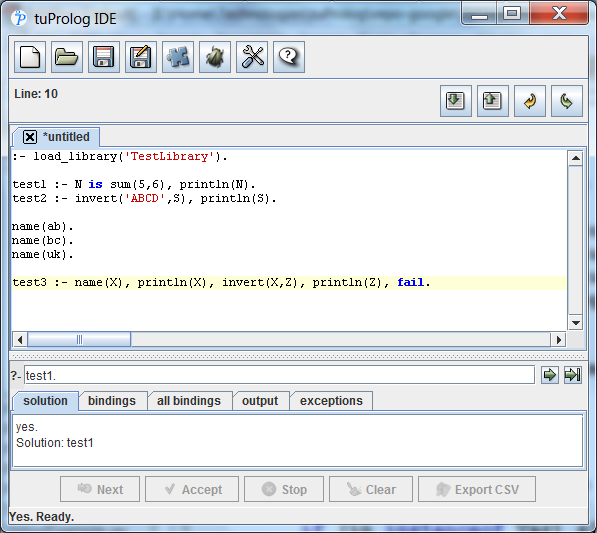
\includegraphics[width=10cm]{images/TestLibrary3}
  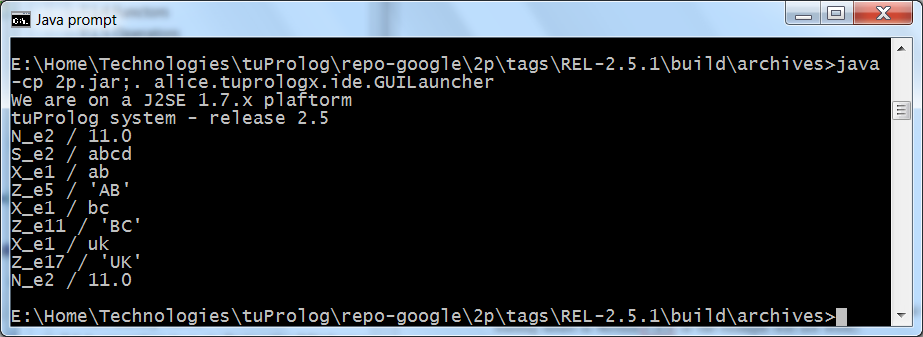
\includegraphics[width=12cm]{images/TestLibrary4}
  \caption{Loading a library from the Prolog side in the GUI \textit{(top)} and its output (\textit{bottom}). Be sure to read the loading issues in Section \ref{ssec:library-loading-issues}, or the example will not work.}
  \label{fig:testlibrary3}
\end{figure}
%
\begin{figure}
    \centering
  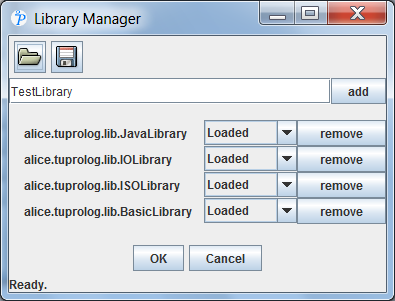
\includegraphics[width=9cm]{images/TestLibrary1}
  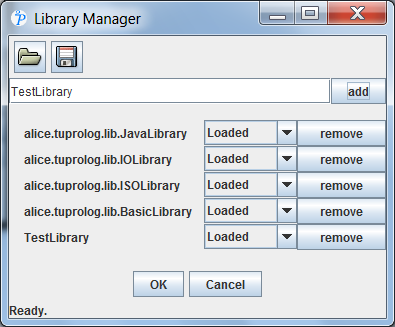
\includegraphics[width=9cm]{images/TestLibrary2}
  \caption{Loading a library from the Prolog side via the Library Manager icon in the \tuprolog{} GUI. The loading issues in Section \ref{ssec:library-loading-issues} still apply. Please note that the browse/save buttons in the dialog are \textit{not} to be used to load/save libraries, but only to load/save \textit{\tuprolog{} preferences} in the form of \texttt{.2p} files.}
  \label{fig:testlibrary1}
\end{figure}
%
\begin{figure}
    \centering
  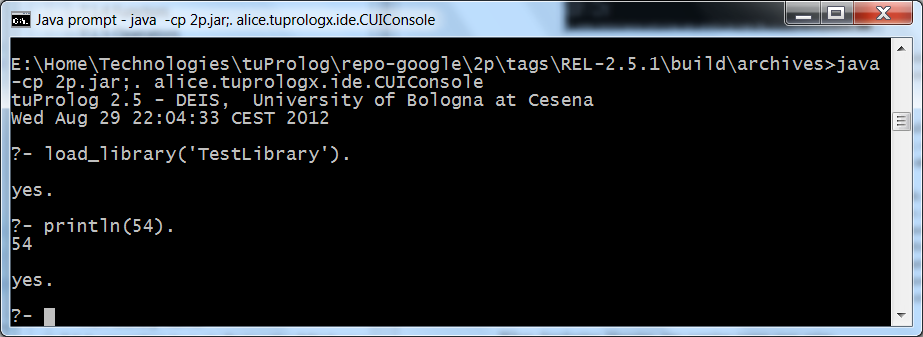
\includegraphics[width=12cm]{images/TestLibrary5}
  \caption{Loading a library from the Prolog side on the CUIConsole: the output here is in the same terminal, as expected. Again, be sure to read the loading issues in Section \ref{ssec:library-loading-issues}, or the example will not work.}
  \label{fig:testlibrary5}
\end{figure}


\subsubsection{Naming issues}

\noindent When developing libraries, two naming issues may arise:
\begin{enumerate}
  \item the name of the predicate, functor or directive should contain a symbol that cannot legally appear in a Java method's name;
  \item a predicate and a directive with the same Prolog signature should be defined, but Java would not be able to distinguish method signatures differing for the return type only.
\end{enumerate}

\noindent To overcome these issues, a \textit{synonym map} must be set up, that maps the desired Prolog names onto legal Java method names, bypassing the standard naming convention.
%
This map must have the form of an array of \texttt{String} arrays, and be returned by the ad hoc \texttt{getSynonymMap} method (abstract in the base \texttt{Library} class).
%
For instance, an evaluable functor \texttt{+}, which cannot appear in a
Java method name, could be implemented by a defining a Java method with any name (say, \texttt{add}) and then map it onto the Prolog name by adding the array \texttt{\{"+", "add", "functor"\}} to the synonym map.

Libraries can also inherit from each other: a library can well extend a user library instead of the base \texttt{Library}, as in the case of the \texttt{HybridLibrary} discussed in the next Section.

%---------------------------------------------------------------
\subsection{Hybrid Java+Prolog libraries}
\label{ssec:hybrid-libraries}
%---------------------------------------------------------------

\begin{table}
    \begin{center}{\tt
    \begin{tabular}{p{12cm}}\hline
    \\
    public class HybridLibrary extends TestLibrary \{\\
    ~public String getTheory()\{\\
    ~~return "myprint(X) :- println(X).$\backslash$n" +\\
    ~~~~~~~~~"myprint(X) :- invert(X,Y), myprint(Y).$\backslash$n";\\
    ~\}\\
    \} \\
    \\
    \hline
    \\
    import alice.tuprolog.*;\\
    import alice.tuprolog.lib.*;\\
    \\
    public class HybridLibraryMain \{\\
    ~~public static void main(String[] args) throws Exception \{\\
	~~~~Prolog engine = new Prolog();\\
	~~~~Library lib2 = engine.loadLibrary("HybridLibrary");\\
	~~~~SolveInfo res = engine.solve("myprint(henry).");\\
	~~~~int count=0;\\
	~~~~while (engine.hasOpenAlternatives() \&\& count < 5)\{\\
	~~~~~~~~count++;\\
	~~~~~~~~res = engine.solveNext();\\
	~~~~\}\\
    \\
    \textrm{\textit{OUTPUT PRINTED:}}\\
    Lib2  LOADED\\
	X\_e1 / henry\\
	X\_e5 / yrneh\\
	X\_e9 / henry\\
	X\_e11 / yrneh\\
	X\_e13 / henry\\
	X\_e15 / yrneh\\
    \\\hline
    \end{tabular}
    }\end{center}
    \caption{A hybrid (mixed) Java + Prolog library \textit{(top)} and the corresponding test program \textit{(bottom)}. }
    \label{tab:HybridLibrary}
\end{table}

Since Java does not support non-determinism, a Java-only library is inherently
deterministic: however, non-determinism can be achieved via hybrid Java + Prolog
libraries, adding a %non-deterministic
Prolog layer on top of the %deterministic
Java layer.

To this end, a library can include a new piece of Prolog theory, embedded into the \texttt{getTheory} method.
%
This method returns a string\footnote{%
    In principle, only the external representation of this theory is constrained to the \texttt{String} form, the internal implementation being up to the developer; yet, using a Java \texttt{String} for wrapping the Prolog code guarantees self-containment while loading libraries through remote mechanisms such as RMI, and therefore constitutes the suggested form.
} (empty by default) containing the desired Prolog theory, and is automatically called when the library is loaded, so as to add the theory to the engine's configuration.

Table \ref{tab:HybridLibrary} shows a hybrid library where the theory in \texttt{getTheory} adds to \texttt{TestLibrary} the non-deterministic predicate \texttt{myprint/1}, whose (potentially infinite) solutions alternately print the argument in upper and lowercase.

%---------------------------------------------------------------
\subsection{Library loading issues}
\label{ssec:library-loading-issues}
%---------------------------------------------------------------

As shown in the above examples, a library can be loaded (and unloaded) dynamically into a running engine via Java, by means of the \texttt{loadLibrary} (\texttt{unloadLibrary}) methods; but it can also be loaded (unloaded) from Prolog, via the \texttt{load\_library/1} (\texttt{unload\_library/1} ) predicate.

Effective from \tuprolog{} 2.6, an enhanced class loading mechanism -- a custom extension to the URLClassLoader -- has been implemented, which overcomes the limitations of the default java class loader that affected the previous \tuprolog{} versions.

In fact, until \tuprolog{} 2.5, starting the \tuprolog{} GUI by double-clicking \texttt{2p.jar} (or by the equivalent \texttt{java -jar} command) prevented libraries from being found and loaded from Prolog via the \texttt{load\_library/1} predicate or via the Library Manager in the GUI, except for the standard libraries packed into the \tuprolog{} JAR itself: this was due to the Java class loader, which would refuse to load classes outside the \textit{runnable} JAR from which the application was started (or from the path specified in its inner manifest file).\footnote{Specifying the \texttt{-cp} option would not work, since Java ignores it in favor of the JAR manifest properties, leading to a runtime failure.}
The suggested workaround was to \textit{avoid} launching \tuprolog{} as a runnable JAR (or by the equivalent \texttt{java -jar} command), in favour of a standard execution via the java interpreter, as follows:\\

\noindent \texttt{~java -cp MyLibrary.jar:2p.jar alice.tuprologx.ide.GUILauncher}\\

\noindent \texttt{~java -cp MyLibrary.jar:2p.jar alice.tuprologx.ide.CUIConsole}\\

\noindent This approach allowed the \texttt{-cp} option to be taken into account by the Java class loader, making it possible to add a specific reference to the library to be loaded (e.g. \texttt{MyLibrary.jar} above), preventing the failure.

In \tuprolog{} 2.6, instead, the new \texttt{load\_library/2} predicate has been added, which takes the desired path list as an extra argument, making it possible to load libraries from virtually anywhere in the file system:

\texttt{?- load\_library('TestLibrary',}\\
\texttt{\mbox{~~~~~~}['C:/Users/Johnny/Desktop/TestProject/test',}\\
\texttt{\mbox{~~~~~~~}'D:/MyLibrary.jar']).}

\noindent Clearly, both the \texttt{'/'} and the \texttt{$\backslash$} file separators are supported, based on the execution platform.

The Library Manager in the \tuprolog{} GUI, shown in Section \ref{ssec:dynamic-library-management}, also takes into account such paths: in fact, if a library file is located in the file system via the \textit{Browse} button, the corresponding path is automatically added to the path list so that the library can be successfully loaded.

As a last remark, the enhanced class loading mechanism implemented in \tuprolog{} 2.6 also applies to the proper JavaLibrary predicates, which now not only search for class files in all the paths specified via the \texttt{set\_classpath} predicates (instead of being limited to the \tuprolog{} JAR), but also accept a path list as an optional extra argument: more on this in Section


%---------------------------------------------------------------
\subsection{Library Name}
\label{ssec:library-name}
%---------------------------------------------------------------

The concept of library name is introduced in \tuprolog{} to separate the physical class name of a library from its logical name, both for clarity -- the library name can be shorter and more meaningful -- and to support multiple versions of the same library, enabling the dynamic upgrade of a library implementation.

By default, the library name is identical to the class name: however, a library can specify a different name by overriding the \texttt{getName} method.
%
Obviously, the full class name is always needed when loading the library, while the library name is used by \texttt{getLibrary} (and similar predicates) to return references to already-loaded libraries.

As an example, in Table \ref{tab:StringLibrary-NewStringLibrary} the \texttt{NewStringLibrary} class provides an alternate implementation of \texttt{StringLibrary}: this is why it \texttt{getName} is redefined so as to return \texttt{StringLibrary} as the \texttt{NewStringLibrary} library name.

\begin{table}
    \begin{center}{\tt
    \begin{tabular}{p{13.5cm}}\hline
    \\
    \mbox{~~~~}public class StringLibrary extends Library \{\\
    \mbox{~~~~~~~~}public boolean to\_lower\_case\_2(Term source, Term dest)\{\\
    \mbox{~~~~~~~~~~~~}String st = source.toString().toLowerCase();\\
    \mbox{~~~~~~~~~~~~}return unify(dest, new Struct(st));\\
    \mbox{~~~~~~~~}\}\\
    \mbox{~~~~~~}\ldots\\
    \mbox{~~~~~~}\textit{// the inherited getName returns "StringLibrary"}\\
    \mbox{~~~~~~}\ldots\\
    \mbox{~~~~}\}\\
    \\
    \hline
    \\
    \mbox{~~~~}public class NewStringLibrary extends Library \{\\
    \mbox{~~~~~~}public String getName()\{ return "StringLibrary"; \}\\
    \mbox{~~~~~~}\ldots\\
    \mbox{~~~~}\}\\
    \\
    \hline
    \end{tabular}
    }\end{center}
    \caption{Defining a new library with the same name as another.}
    \label{tab:StringLibrary-NewStringLibrary}
\end{table}


%-----------------------------------------------------------------------
\section{Augmenting Java via Prolog:\\the P@J framework}
\label{sec:p@j}
%-----------------------------------------------------------------------

The last dimensions of \tuprolog{}'s support to multi-paradigm, multi-language programming is still a form of \textit{augmenting} a language (that is, exploiting a language and a paradigm to increase the other)---in this case, augmenting Java from Prolog, exploiting the so-called \textit{P@J} framework \cite{short-patj-sac08}.

This approach makes it possible to ``inline intelligence'' into Java code, enabling Prolog to be used for implementing Java (abstract) methods, via Java reflection and suitable annotations.
%
The basic idea is that the methods to be implemented in Prolog are declared
\texttt{abstract} from the Java syntax viewpoint\footnote{%
  Of course, the corresponding class must be syntactically qualified \texttt{abstract}, too.
}, so that the Java compiler does not expect to find any implementation, while annotating them with the Prolog clauses that provide the actual implementations.
On the user side, the factory method \texttt{PJ.newInstance} will be used to automatically create a Java implementation of this method, which interacts with the Prolog engine in a totally transparent way.

The technique relies on advanced features of Java such generic types, wildcards, and type inference, as well as reflection to ``put things together''; for this reason, some syntax conventions are required for method signatures:
\begin{itemize}
  \item the Prolog predicate name must be identical to the Java method name;

  \item the argument types must be explicitly declared each with the corresponding bounding, and their names must start with \texttt{\$};

  \item the argument position in the Java method signature must reflect their role as input or output arguments in the Prolog predicate: the first are to be put in the argument list, and the latter in the return type.
\end{itemize}

\noindent The last requirement is necessary to bridge between the Prolog predicate syntax, where both input and output arguments are in the argument list (with nothing explicitly qualifying these roles, according to the declarative nature of the language), and the Java method syntax, where the only output argument is not in the argument list, but is ``returned from'' the method.

%---------------------------------------------
\subsection{Term taxonomy}
\label{ssec:p@j-term-taxonomy}
%---------------------------------------------

Here, too, a suitable taxonomy is needed to map the relevant Prolog types (term, atom, number, list, variable, etc) in Java; however, while the domain to represent is the same as above (Section \label{ssec:java-api-types}), the requirements due to type inference and strong type checking made it necessary to define one further, \textit{ad hoc} taxonomy as the base of the annotation layer.

The new hierarchy exploits the basic types in Figure \ref{fig:term-taxonomy} on page \pageref{fig:term-taxonomy} as its building bricks, and builds a new layer on top.
The new root is the abstract class \texttt{Term<X>}, whose definition exploits a recursive pattern to reify (represent) the type of the actual term content:

\begin{verbatim}
   abstract class Term<X extends Term<?>> {..}
\end{verbatim}

\noindent Accordingly, the term subclasses are defined as:

\begin{verbatim}
 class Atom extends Term<Atom> {..}
 class Int extends Term<Int> {..}
 class Double extends Term<Double> {..}
 class List<X extends Term<?>> extends Term<List<X>> {..}
 ...
\end{verbatim}

\noindent where, clearly, \texttt{Term<Int>} is used for a term containing an \texttt{Int}, \texttt{Term<Double>} for a term containing a \texttt{Double}, \texttt{Term<List<Int>>} for a term containing a \texttt{List<Int>}, etc.

Variables are a notable exception, because they must be able to contain values of the above types: for this reason, \texttt{Var<X>} is \textit{not} defined as a subtype of \texttt{Term<Var<X>>}, but directly of \texttt{Term<X>}.

\begin{verbatim}
 class Var<X extends Term<?>> extends Term<X> {..}
\end{verbatim}

\noindent As a consequence, both types \texttt{X} and \texttt{Var<X>} derive from the common ancestor Term<X>, which makes it possible to represent method arguments that may be a logical input or output---i.e., that must accept both a value (a term of type \texttt{X}) or a variable (a term of type \texttt{Var(X)}).

Thanks to this approach, a method definition like the following:

\begin{verbatim}
 boolean length(Term<? extends List<?>> list, Term<Int> size)
\end{verbatim}

\noindent can be read as follows:

\begin{itemize}
  \item list is a term containing any list, and size is an integer;

  \item both arguments can be either input or output.
\end{itemize}

\noindent The term hierarchy is completed by the \texttt{Compound} term family, which enables the definition of compound terms of any arity by means of a list-like approach---that is, starting from the empty compound term \texttt{Nil} and building bigger compounds with the \texttt{Cons} class constructor.
However, shortcut classes \texttt{Compound1}, \texttt{Compound2} and \texttt{Compound3} are provided for the user convenience to specify the most common terms of 1, 2 or 3 arguments:

\begin{verbatim}
 public abstract class Compound<X extends Compound<?>>
   extends Term<X> {..}

 public class Cons<H extends Term<?>, R extends Compound<?>>
   extends Compound<Cons<H,R>> implements Iterable<Term<?>>{..}

 public class Nil extends Compound<Nil> {..}

 public class Compound1<X1 extends Term<?>>
   extends Cons<X1,Nil> {..}

 public class Compound2<X1 extends Term<?>, X2 extends Term<?>>
   extends Cons<X1,Cons<X2,Nil>> {..}

 public class Compound3<X1 extends Term<?>, X2 extends Term<?>,
                        X3 extends Term<?>>
   extends Cons<X1,Cons<X2,Cons<X3,Nil>>> {..}
\end{verbatim}

%---------------------------------------------
\subsection{Examples}
\label{ssec:p@j-examples}
%---------------------------------------------

As an example, Table \ref{tab:pj-example1} shows a Java class \texttt{Perm} with the \texttt{permutation} method implemented in Prolog.
%
The Java method declaration specifies that there is one input argument and one output argument: the first (\texttt{\$X}) is a \texttt{List<Int>} (or a covariant type), the second (\texttt{\$Y}) is an \texttt{Iterable} over a \texttt{List<Int>} (or a covariant type).
The \texttt{Iterable} specification is needed to iterate over all solutions: if only the first solution is needed, \texttt{\$Y} could have been used instead of \texttt{Iterable<\$Y>}.

Moreover, since arguments are declared in the order (\texttt{\$X}), (\texttt{\$Y}) in the Java method signature, they will be mapped in this order on the Prolog predicate arguments: so (\texttt{\$X}) will map onto the first argument of \texttt{permutation/2}, and (\texttt{\$Y}) on the second argument.

In the client program, the \texttt{Perm} instance \texttt{p} is created indirectly via the \texttt{PJ.newInstance} factory method, whose argument is the corresponding \texttt{Class} meta-class, \texttt{Perm.class}.
Then, the \texttt{p} object can be used normally, like any other Java object: here it computes all the permutations of a given list of integers (built from an array, just to play with types), which is then iterated over by a \textit{for-each} loop that prints every result.
The actual type for both \texttt{\$X} and \texttt{\$Y}, \texttt{List<Int>}, is inferred automatically by the P@J runtime.

\begin{table}
{\footnotesize
\begin{tabular}[-1cm]{p{12cm}}
\begin{verbatim}
import alice.tuprologx.pj.annotations.*;
import alice.tuprologx.pj.engine.*;
import alice.tuprologx.pj.model.*;
import alice.tuprologx.pj.meta.*;
import java.util.List;
import java.util.ArrayList;
\end{verbatim}
\textsf{\emph{A Java class augmented via Prolog}}
\begin{verbatim}
abstract class Perm{
    @PrologMethod ( clauses = {
        "permutation([],[])." ,
        "permutation(U,[X|V]):-remove(U,X,Z),permutation(Z,V)." ,
        "remove([X|T],X,T)." ,
        "remove([X|U],E,[X|V]):-remove(U,E,V)."
        }
    )
    public abstract < $X extends List<Int>, $Y extends List<Int> >
                Iterable<$Y> permutation($X list);
}
\end{verbatim}
\textsf{\emph{A sample client class}}
\begin{verbatim}
public class PJexample {
  public static void main(String[] args) throws Exception {
    java.util.Collection<Integer> v = java.util.Arrays.asList(1,2,3);
    Perm p=PJ.newInstance(Perm.class);
    for (List<Int> list : p.permutation(new List<Int>(v))) {
        System.out.println(list.toJava());
    }
  }
}
\end{verbatim}
\textsf{\emph{Output printed:}}
\begin{verbatim}
    [1, 2, 3]
    [1, 3, 2]
    [2, 1, 3]
    [2, 3, 1]
    [3, 1, 2]
    [3, 2, 1]
\end{verbatim}
\end{tabular}
}\caption{A Java class exploiting Prolog for implementing an abstract method \textit{(top)} and a client using it \textit{(bottom)}. Note that the \texttt{Arrays.asList} method exploits the Java shortcut syntax for varargs.
To run the example, the \texttt{javassist.jar} library, used by the P@J runtime, must be in the class path: \texttt{E:>java~~-cp .;2p.jar;javassist.jar PJexample}
}
\label{tab:pj-example1}
\end{table}


\begin{table}
{\footnotesize
\begin{tabular}[-1cm]{p{12cm}}
\begin{verbatim}
import alice.tuprologx.pj.annotations.*;
import alice.tuprologx.pj.engine.*;
import alice.tuprologx.pj.model.*;
import alice.tuprologx.pj.meta.*;
\end{verbatim}
\textsf{\emph{Another Java class augmented via Prolog}}
\begin{verbatim}
@PrologClass(
	clauses = {"size(X,Y) :- length(X,Y)."}
)
public abstract class PJLength {	
    @PrologMethod abstract <$Ls extends List<?>, $Ln extends Int>
    Boolean size($Ls expr, $Ln rest);
    @PrologMethod abstract <$Ls extends List<?>, $Ln extends Int>
    $Ln size($Ls expr);
    @PrologMethod abstract <$Ls extends List<?>, $Ln extends Int>
    $Ls size($Ln expr);
    @PrologMethod abstract <$Ls extends List<?>, $Ln extends Int>
    Iterable<Compound2<$Ls,$Ln>> size();

    public static void main(String[] args) throws Exception {
        PJLength pjl = PJ.newInstance(PJLength.class);
        java.util.List<?> v = java.util.Arrays.asList(12,"ok",false);
        List<?> list = new List<Term<?>>(v);
        Boolean b = pjl.size(list, 3);   // true
        Int i = pjl.size(list);          // length is 3
        List<?> l = pjl.size(3);         // produces [_,_,_]
        int cont = 0;
        for (Term<?> t : pjl.size()) {   // [],[_],...,[_,_,_,_,_]
            System.out.println(t);
            if (cont++ == 5) break;
        }
    }
}\end{verbatim}
\textsf{\emph{Output printed:}}
\begin{verbatim}
    Compound:'size'(List[],Int(0))
    Compound:'size'(List[Var(_)],Int(1))
    Compound:'size'(List[Var(_), Var(_)],Int(2))
    Compound:'size'(List[Var(_), Var(_), Var(_)],Int(3))
    Compound:'size'(List[Var(_), Var(_), Var(_), Var(_)],Int(4))
    Compound:'size'(List[Var(_), Var(_), Var(_), Var(_), Var(_)],Int(5))
\end{verbatim}
\end{tabular}
}\caption{Another Java class exploiting Prolog for method implementation. The \texttt{length/2} predicate used in the \texttt{clauses} section on top is part of the standard ISO list management predicates.}
\label{tab:pj-example2}
\end{table}

\begin{table}
{\footnotesize
\begin{tabular}[-1cm]{p{12cm}}
\begin{verbatim}
import alice.tuprologx.pj.annotations.*;
import alice.tuprologx.pj.engine.*;
import alice.tuprologx.pj.model.*;
import alice.tuprologx.pj.meta.*;
\end{verbatim}
\textsf{\emph{Another Java class augmented via Prolog}}
\begin{verbatim}
@PrologClass (
  clauses={"arc(a,b)." , "arc(a,d)." , "arc(b,e)." , "arc(d,g).",
           "arc(g,h)." , "arc(e,f)." , "arc(f,i)." , "arc(e,h)."}
)
public abstract class PJPath {
  @PrologMethod (
    clauses = {	"path(X,X,[X]).",
                "path(X,Y,[X|Q]):-arc(X,Z),path(Z,Y,Q)."}
  )
  public abstract <$X,$Y,$P> Iterable<$P> path($X from, $Y to);

  public static void main(String[] s) throws Exception {
    PJPath pjp = PJ.newInstance(PJPath.class);
    for (Object solution : pjp.path(new Atom("a"), new Var<Atom>("X"))) {
      System.out.println(solution);
    }
  }
}\end{verbatim}
\textsf{\emph{Output printed:}}
\begin{verbatim}
  List[Atom(a)]
  List[Atom(a), Atom(b)]
  List[Atom(a), Atom(b), Atom(e)]
  List[Atom(a), Atom(b), Atom(e), Atom(f)]
  List[Atom(a), Atom(b), Atom(e), Atom(f), Atom(i)]
  List[Atom(a), Atom(b), Atom(e), Atom(h)]
  List[Atom(a), Atom(d)]
  List[Atom(a), Atom(d), Atom(g)]
  List[Atom(a), Atom(d), Atom(g), Atom(h)]
\end{verbatim}
\end{tabular}
}\caption{Another Java class exploiting Prolog for method implementation.}
\label{tab:pj-example3}
\end{table}


Two further examples are shown in Table \ref{tab:pj-example2} and Table \ref{tab:pj-example3}, respectively.
The first operates on lists, and finally generates (and prints) five ``lists of anything'' of 1,2,3,4,5 arguments; the second computes the path between two given nodes in a graph. In both cases, Prolog is delegated the reasoning part, while Java is exploited as the front-end to the user.
Technically, attention is required to distinguish Java lists (i.e., instances of \texttt{java.util.List} and its subclasses) from P@J \texttt{List}, which handles terms like \texttt{Term<X>}; moreover, the example in Table \label{tab:pj-example2} shows the inner structure of compounds.

For completeness, Table Table \ref{tab:pj-example4} shows a last, more complex example, where the Prolog code specifies a parser for arithmetic expressions.

\begin{table}
{\footnotesize
\begin{tabular}[-1cm]{p{12cm}}
\begin{verbatim}
import alice.tuprologx.pj.annotations.*;
import alice.tuprologx.pj.engine.*;
import alice.tuprologx.pj.model.*;
import alice.tuprologx.pj.meta.*;

@PrologClass
public abstract class PJParser {
  @PrologMethod (clauses={"expr(L,R):-term(L,R).",
                          "expr(L,R):-term(L,['+'|R2]), expr(R2,R).",
                          "expr(L,R):-term(L,['-'|R2]), expr(R2,R)."})
  public abstract <$E extends List<?>, $R extends List<?>>
  Boolean expr($E expr, $R rest);

  @PrologMethod (clauses={"term(L,R):-fact(L,R).",
                          "term(L,R):-fact(L,['*'|R2]), term(R2,R).",
                          "term(L,R):-fact(L,['/'|R2]), term(R2,R)."})
  public abstract <$T extends List<?>, $R extends List<?>>
  Boolean term($T term, $R rest);
	
  @PrologMethod (clauses={"fact(L,R):-num(L,R).",
                          "fact(['(' | E],R):-expr(E,[')'|R])."})
  public abstract <$F extends List<?>, $R extends List<?>>
  Boolean fact($F fact, $R rest);
	
  @PrologMethod (clauses={"num([L|R],R):-num_atom(_,L)."})
  public abstract <$N extends List<?>, $R extends List<?>>
  Boolean num($N num, $R rest);
	
  public static void main(String[] args) throws Exception {
    PJParser ep = PJ.newInstance(PJParser.class);
    String tokenizer_regexp =
      "(?<!^)(\\b|(?=\\()|(?=\\))|(?=\\-)|(?=\\+)|(?=\\/)|(?=\\*))";
    List<Atom> exp1 = new Atom("12+(3-4)").split(tokenizer_regexp);
    List<Atom> exp2 = new Atom("(12+(3-4))").split(tokenizer_regexp);
    System.out.println(ep.expr(exp1, List.NIL)); // 12+(3*4)   expression ?
    System.out.println(ep.fact(exp1, List.NIL)); // 12+(3*4)   factor ?
    System.out.println(ep.expr(exp2, List.NIL)); // (12+(3*4)) expression ?
    System.out.println(ep.fact(exp2, List.NIL)); // (12+(3*4)) factor ?
  }
}\end{verbatim}
\end{tabular}
}\caption{A parser for arithmetic expressions encoded in Prolog inside an annotated Java program. The output prints \texttt{true}, \texttt{false}, \texttt{true}, \texttt{true} in this order, since 12+(3*4) is an expression but not a factor, while (12+(3*4)) is both an expression and a factor.}
\label{tab:pj-example4}
\end{table}
